%%%%%%%%%%%%%%%%%%%%%%%%%%%%%%%%%%%%%%%% Klasse Festlegen
%\documentclass[Master,MDS,english,fhCitStyle,HARVARD]{BASE/twbook} 
\documentclass[Master,MDS,english]{BASE/twbook} % FH definierte Zitierstandards verwenden 
%%%%%%%%%%%%%%%%%%%%%%%%%%%%%%%%%%%%%%%% Verwendete Packages
\usepackage[utf8]{inputenc} % Zeichen-Enkodierung (evtl. Abweichungen für Apple)
\usepackage[T1]{fontenc}    % Zeichen-Enkodierung
\usepackage{blindtext}      % Platzhaltertexte
\usepackage{minted}         % Darstellung von Code
\usepackage{comment}        % Auskommentieren von ganzen Passagen
\usepackage{csquotes}
\usepackage{algorithm}      % Umgebung f Algorithmen
\usepackage[noend]{algpseudocode}
                            % Wenn Sie während Ihrer Arbeit
                            % merken, dass Sie zusätzliche Funktionen
                            % benötigen ist hier ein guter Platz um
                            % weitere Packages zu laden
%%%%%%%%%%%%%%%%%%%%%%%%%%%%%%%%%%%%%%%% Zitierstil zum selbst definieren
%\usepackage[backend=biber, style=ieee]{biblatex}            % LaTeX definierter IEEE- Standard
%\usepackage[backend=biber, style=authoryear]{biblatex}      % LaTeX definierter Harvard-Standard
\usepackage{cite}
\usepackage[round]{natbib}
\usepackage{subcaption}
\usepackage{multirow}
\usepackage{siunitx}
\usepackage{geometry}
\usepackage{booktabs}
\usepackage{multirow}
\usepackage{microtype} 
%\usepackage{algorithm}
%\usepackage{algorithmic}
\captionsetup{compatibility=false}

%\addbibresource{Literatur.bib}                              % Literatur-File definieren
%%%%%%%%%%%%%%%%%%%%%%%%%%%%%%%%%%%%%%%% Einträge für Deckblatt
\title{Multi-sensor rail track detection \\ in automatic train operations}

\author{Attila Kovacs}
\studentnumber{2110854031}
%\author{Titel Vorname Name, Titel\and{}Titel Vorname Name, Titel}
%\studentnumber{XXXXXXXXXXXXXXX\and{}XXXXXXXXXXXXXXX}

\supervisor{Lukas Rohatsch}
%\supervisor[Begutachter]{Titel Vorname Name, Titel}
%\supervisor[Begutachterin]{Titel Vorname Name, Titel}
\secondsupervisor{Daniele Capriotti}
%\secondsupervisor[Begutachter]{Titel Vorname Name, Titel}
%\secondsupervisor[Begutachterinnen]{Titel Vorname Name, Titel}

\place{Wien}
%%%%%%%%%%%%%%%%%%%%%%%%%%%%%%%%%%%%%%%% Danksagung/Kurzfassung/Schlagworte
\kurzfassung{Die Erhöhung des Automatisierungsgrades im Bahnbetrieb ist ein Schlüsselfaktor für die Erreichung eines effizienteren und wettbewerbsfähigeren Eisenbahnsystems. Automatische Zugbetriebssysteme (ATO) nutzen fortschrittliche Technologien, um die Eisenbahnumgebung wahrzunehmen und zu interpretieren und um autonome Betriebsabläufe mit minimalem menschlichem Eingriff zu ermöglichen. Die präzise Identifizierung und Lokalisierung von Eisenbahngleisen sind grundlegend für eine sichere Zugnavigation. Daher besteht Bedarf an robusten automatisierten Methoden zur Gleiserkennung.

Diese Masterarbeit befasst sich mit der Aufgabe der Mehrsensorschienenverfolgung im Rahmen von ATO durch die Nutzung von Deep-Learning-Techniken, insbesondere der semantischen Segmentierung. Durch die Erforschung eines Mehrsensordatensatzes, der Bilder von hoch-/niedrigauflösenden RGB-Kameras und Infrarotkameras mit unterschiedlichen Orientierungen umfasst, zielt diese Forschung darauf ab die Genauigkeit und Robustheit der Gleiserkennung unter verschiedenen Bedingungen zu verbessern. Die Studie vergleicht die Leistung der Deep-Learning-basierten Segmentierung mit traditionellen nicht-KI-basierten Methoden, führt umfassende Bewertungen verschiedener Sensorinputs durch und erforscht die Integration in realen Anwendungen. Die Ergebnisse liefern wertvolle Erkenntnisse auf dem Gebiet der Eisenbahnautomatisierung und bieten Implikationen zur Verbesserung der Sicherheit und Effizienz des automatischen Zugbetriebs.}




\schlagworte{Deep Learning, Computer Vision, Segmentation, Automatic Train Operations}
\outline{Increasing the level of automation in train operations is an enabler for achieving a more efficient and competitive railway system. Automatic train operations (ATO) systems use advanced technologies to perceive and interpret the railway environment in order to facilitate autonomous operations with minimal human intervention. Precise identification and localization of railway tracks are fundamental for safe train navigation. Hence there is a need for robust automated track detection methods. 

This master's thesis addresses the task of multi-sensor rail track detection within the ATO framework by utilizing deep learning techniques, particularly semantic segmentation. By exploring a multi-sensor dataset comprising images from high/low-resolution RGB cameras and infrared cameras with varying orientations, this research aims to improve the accuracy and robustness of track detection in diverse conditions. The study compares the performance of deep learning-based segmentation with traditional non-AI-based methods, conducts comprehensive evaluations on different sensor inputs, and explores real-world application integration. The findings contribute valuable insights to the field of railway automation, offering implications for enhancing the safety and efficiency of automatic train operations.}
\keywords{Deep Learning, Computer Vision, Rail Track Segmentation, YOLO, Automatic Train Operations}
\acknowledgements{The author would like to thank Lukas Rohatsch and Daniele Capriotti for their support and insightful contributions. Acknowledgment is also extended to DB and DB Cargo for providing the essential images and videos that made this research possible. 
The computational infrastructure was graciously provided by the UAS Technikum Wien.
}
\setListingsAndAcronyms % Definition der Namen für Quellcodeverzeichnis 
%%%%%%%%%%%%%%%%%%%%%%%%%%%%%%%%%%%%%%%% Ende des Headers
%%%%%%%%%%%%%%%%%%%%%%%%%%%%%%%%%%%%%%%% Beginn des Dokuments
\begin{document}
%%%%%%%%%%%%%%%%%%%%%%%%%%%%%%%%%%%%%%%% 
\maketitle
%%%%%%%%%%%%%%%%%%%%%%%%%%%%%%%%%%%%%%%% Beginn des Inhalts

\chapter{Introduction} %500 words


According to the International Energy Agency (IEA), the global demand for passenger and freight transportation will more than double by 2050 compared to 2019 \citep{IEA2019}. However, a greater demand entails higher energy consumption as well as increased CO2 emissions and atmospheric pollutants.  
Given the fact that railway is one of the most efficient and reliable modes of transportation, there seems to be consensus between politicians and researchers that a greater share of rail transportation has the potential to counterbalance the negative impacts of transportation \citep{islam2016make, pagand2020fostering}.
The IEA lists minimizing costs per passenger-kilometer or ton-kilometer moved as one of three pillars that are essential to increase the market share of rail transportation\footnote {The other pillars are maximizing revenues from rail systems and ensuring that all forms of transport (especially road transportation) pay not only for the use of the infrastructure they need, but also for the adverse impacts they generate.}.

Automatic Train Operations (ATO) which refers to a system that automates different aspects of train operations is expected be one of the key drivers of a more efficient and competitive railway system \citep{ERJU2019, ALSTOM2021}. ATO is estimated to reduce energy consumption by up to 45\%, increase the level of punctuality, increase operational flexibility, and allow for a 50\% better utilization of the infrastructure when combined with other technologies.

ATO relies on advanced technologies that are used to perceive and interpret the railway environment in order to allow autonomous operations with minimal or no human intervention \citep{DB2024}. 
One aspect of ATO is the precise identification and localization of railway tracks. The ability to detect and isolate tracks based on video images is essential for ensuring the safe navigation of trains through the railway network or in shunting yards. Accurate track detection ensures that the train can make informed decisions, such as adjusting speed, navigating turns, and responding to potential obstacles.

Traditional methods of track detection often rely on rule-based algorithms and image processing techniques but these approaches may face challenges in diverse environmental conditions such as bad weather, complex background, lighting variations (e.g., day and night), and dirty cameras.
This master's thesis addresses the task of multi-sensor rail track detection in the context of ATO. We explore deep-learning techniques, particularly semantic segmentation, that have demonstrated great success in computer vision tasks. The application of deep learning to track detection is expected to outperform conventional non-AI-based techniques and thereby improving the accuracy and robustness of the system.
Our analysis is based on a multi-sensors dataset, including images of normal RGB cameras, high-resolution cameras, and infrared cameras with different orientations, respectively. This multi-sensor approach allows us to compare the effectiveness of different camera types and informs the deployment of those in order to improve the robustness of track detection in diverse conditions. 

In the context of rail track detection, researchers have explored various areas. Yet, applying deep learning techniques to detect rail tracks is a relatively raw field. In particular, there is no research that is focusing on comparing different input images such as RGB and infrared cameras and images that are oriented to the left, center, and right of the locomotive. 
The contribution of this thesis to the literature is three-fold: First, we select and train different deep learning models capable of accurately detecting and segmenting railway tracks using data from RGB cameras, high-resolution cameras, and infrared cameras. In contrast to approaches that have been specifically tailored to the task, we apply a general framework that is easier to use by practitioners without elaborate software engineering skills.
The results of the deep learning model are compared to a non-AI based method specialized in identifying lines in images. 
Second, we conduct a comprehensive performance evaluation to assess the accuracy and computational efficiency of the proposed track detection system on images generated by different cameras.
Third, we explore the integration of the developed model into real-world applications by applying the model to identify tracks in video streams. Within the proposed framework we apply a post-processing step to the segmentation result in order to increase the robustness of the results. 

By achieving these objectives, this research provides valuable insights and advancements to the field of railway automation with implications for improving the safety and efficiency of automatic train operations.




\chapter{Literature review} %1000 words

Traditionally, rail track detection has been performed by first extracting features of an image (e.g., gradient-based thresholds) and then detecting rails. These approaches achieve good results in certain conditions. However, deep-learning based approaches are often more robust in real-world environments \citep{7350873, 8859360, 10.1145/3503161.3548050}.
Deep learning techniques, particularly CNNs, have emerged as powerful tools for image segmentation tasks, demonstrating success in various computer vision applications. Recent surveys on image segmentation and object detection using deep-learning techniques is provided by \cite{cmc.2023.032757} and \cite{ZAIDI2022103514}, respectively.

The following sections examine related research in track detection, considering both deep learning-based segmentation and traditional non-AI segmentation methods.



\section{Traditional rail track detection}

While deep learning has shown remarkable success in track detection, non-AI segmentation techniques continue to play a role in this field as they allow the integration of domain-specific knowledge and rules into the algorithm and require less data for training. These methods are often referred to as line segment detectors and involve traditional computer vision techniques such as thresholding, edge/contour detection, template matching, and region growing \citep{4731268, ipol.2012.gjmr-lsd, 8100103, SAHOO1988233, Mittal2022}.

\cite{5309526} present a dynamic programming algorithm to extract the rail tracks in front of the train. The idea is to first identify the vanishing point which refers to the imaginary intersection of the tracks as the distance between the tracks decreases from the bottom of the image to the top.  This step is based on computing the gradient and applying Hough transform to detect the straight lines that indicate the tracks. Next, dynamic programming is used to extract the space between the two tracks.
 \cite{qi2013efficient} apply a method based on histogram of oriented gradients (HOG) to identify tracks and switches. First, HOG features are computed.  Railway tracks are then identified by a region-growing algorithm. The proposed method is able to predict the patch the train will travel by detecting the setting of the switches. 
\cite{5940410} introduce an approach that performs rail extraction by matching edge features to candidate templates.

While the previously mentioned approaches focus on images by on-board cameras, \cite{7952544} examines the detection of tracks in aerial images taken by drones. The solution approach is based on Hough transform.

\cite{rs71114916} and \cite{6783695} develop methods to recognize railroad infrastructure from 3D LIDAR data.
In \cite{rs71114916}, railway components such as rail tracks, contact cables, catenary cables, masts, and cantilevers are classified based on local neighborhood structure, shape of objects, and topological relationships among objects. 
\cite{6783695} focus on the detection of tracks. The authors utilize the geometry and reflection intensity of the tracks to
extract features and identify tracks.


\section{Deep-learning based rail track detection}

Deep-learning based techniques such as semantic segmentation incorporate convolutional neural networks (CNNs) and other deep architectures to automatically learn features from raw image data. Semantic segmentation aims to assign a label to each pixel in the image, distinguishing between the pixels that belong to the rail tracks and those that represent the background. The approach is therefore particularly well suited for rail track detection. 

\cite{7350873} and \cite{8517865} were among the first authors who evaluated the performance of deep learning-based segmentation against traditional segmentation techniques in rail track detection. 
In \cite{7350873}, the authors propose a CNN for localizing and inspecting the condition of railway component based on gray-scale images. The authors report that the CNN model is better suited to capture complex patters compared to approaches that rely on traditional texture features (e.g., discrete Fourier transforms of local binary pattern histograms). 
\cite{8517865} detect rail tracks in aerial images by devising a CNN based approach and different traditional approaches such as thresholding. 

\cite{8859360} propose the RailNet -- a deep-learning based rail track segmentation algorithm that combines the ResNet50 backbone with a fully convolutional network. In order to train the model, the authors compile a non-public dataset consisting of 3000 images from forward-facing on-board cameras. Experiments show that RailNet is able to outperform general purpose models for segmentation.
\cite{10.1145/3503161.3548050} compile a real-world railway dataset based on which a rail detection method referred to as Rail-Net is devised. Rail-Net outperforms traditional methods by around 51\% and other deep-learning methods by around 6\% based on accuracy when applied on the newly compiled dataset. 

A machine-learning based approach is proposed by \cite{teng2016visual} where features are extracted from super-pixels (i.e., a group of adjacent pixels with similar characteristics) and classified by applying a previously trained support vector machine.


\section{Lane detection} \label{sec:lane_detection}

Lane detection for road vehicles is similar to rail track detection for locomotives in the sense that both tasks aim to identify and segment elongated shapes in complex environments that vary in lighting conditions, shadows, and occlusions. 
The field of lane detection has a rich body of literature which is among others attributed to the existence of well-established benchmark datasets such as \cite{TuSimple} and CULane \citep{pan2018SCNN}. 

Early work on lane detection is based on traditional approaches such as Hough transform and clustering \citep{10.1145/361237.361242, 5432669}. Recently, the focus of researchers has shifted to deep-learning based approaches \citep{meyer2021yolino, zheng2022clrnet, wang2022keypoint}.
\cite{tang2021review} and \cite{yang2023lane} provide comprehensive surveys on lane detection approaches. In \citep{yang2023lane}, the authors propose a combined approach in which the advantages of traditional and deep-learning based methods are mixed.


\chapter{Datasets} %2000 words

Labeled images are an essential prerequisite for training deep-learning algorithms to detect objects accurately.
With the growing popularity of deep-learning, there has been an ongoing effort to create new datasets specifically designed for railway applications.

The rail semantics dataset 2019 (RailSem19) is the first publicly available
dataset for detecting objects (including rail tracks) in the railway domain \citep{9025646}. 
The French railway signaling dataset (FRSign) is a dataset focusing only on traffic lights \citep{9025646}, whereas the Railway Pedestrian Dataset (RAWPED) is focusing on pedestrian detection methods \citep{9050835}. The dataset proposed by \cite{8859360} -- railroad segmentation dataset -- has been compiled for the development of railroad segmentation algorithms but it is not available to the public. The Rail-DB dataset comprises 7.432 annotated images, featuring different scenarios (e.g., weather conditions), and is available upon request \citep{10.1145/3503161.3548050}.  

This thesis is based on the first freely available multi-sensor dataset ``Open Sensor Data for Rail 2023'' (OSDaR23) for the development of fully automated driving in the railway sector \citep{DB2023, tagiew2023osdar23}.
Unlike the previously mentioned dataset that involve a limited number of sensors and perspectives, the system on the locomotive used to create the OSDaR23 dataset includes multiple infrared cameras, RGB cameras with different resolutions, lidar, radar, positioning, and acceleration sensors.

Preliminary experiments indicated that our segmentation model fails to generalize when trained only on the OSDaR23 dataset due to reasons that will be described in the next section. Therefore, we also train our model on images from the RailSem19 dataset.
In the following, we give a detailed description of the two datasets used in this thesis.


\section{OSDaR23 dataset} \label{sec:OSDaR23}

\subsection{Overview}

The OSDaR23 contains 21 video sequences captured around Hamburg, Germany between 09.09.2021 and 15.09.2021 (a map of the exact locations is given in Figure~\ref{fig:map}). 
The sensor setup is comprehensive including six RGB cameras, three
IR cameras, six lidar sensors, a 2D radar sensor, and position and acceleration sensors. In this thesis, we focus on images by RGB high resolution, RGB low resolution, and infrared sensors with three orientation (left, right, and center), respectively. One example per sensor is given in Figure~\ref{fig:sensor_image}. A detailed description of the sensors can be found in Appendix~\ref{app:sensors}.

\begin{figure}[h]
\centering
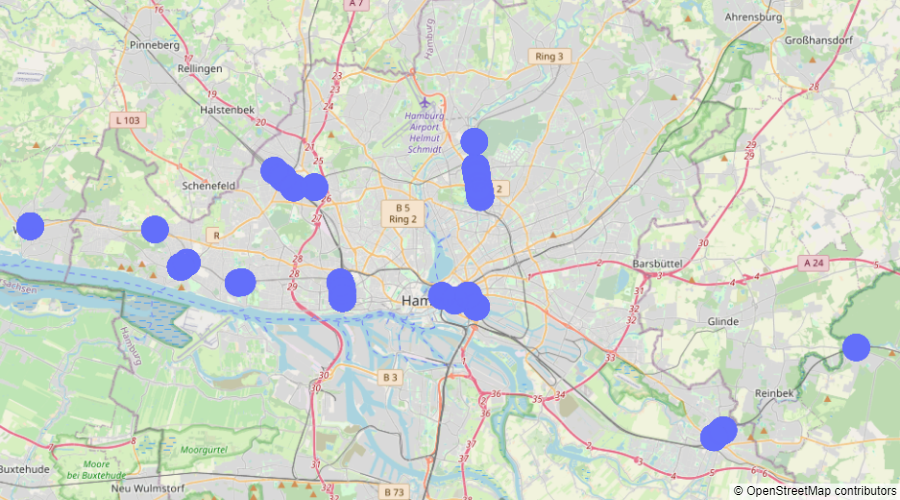
\includegraphics[width=0.5\textwidth]{images/datasets/db/map}
\caption{Locations where images were captured around Hamburg, Germany. }
\label{fig:map}
\end{figure}

\begin{figure}[h]
\centering
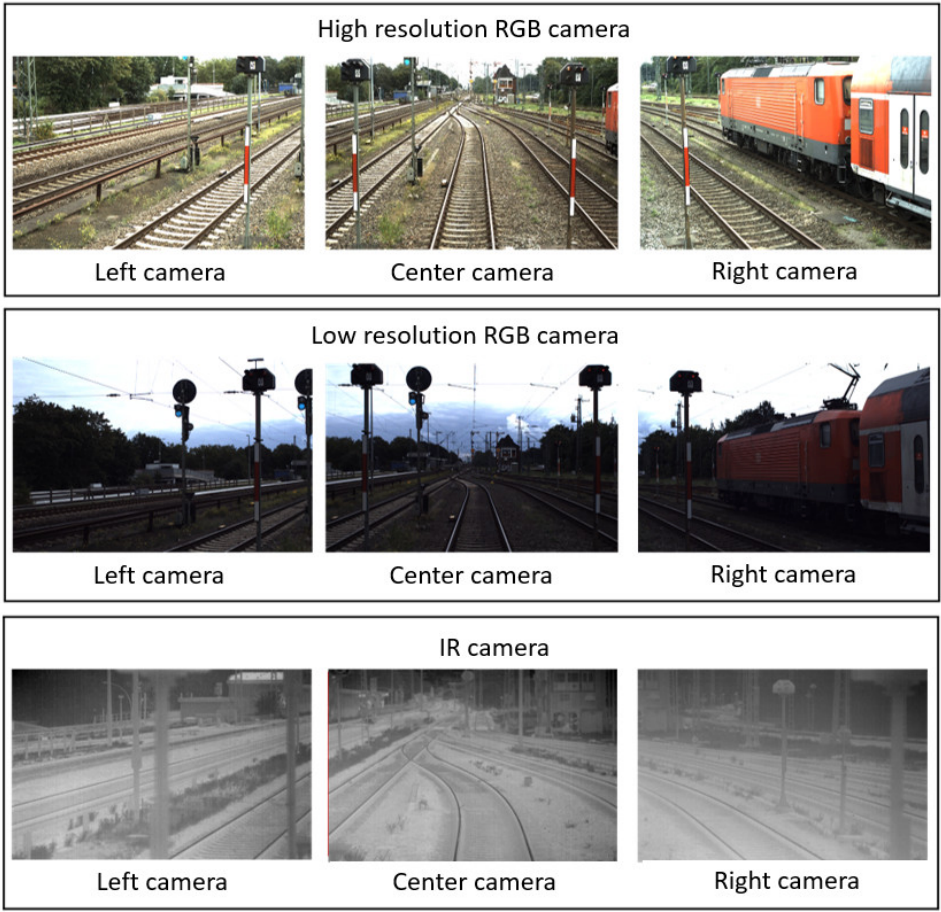
\includegraphics[width=0.5\textwidth]{images/datasets/db/2024-01-29 19_50_46-2305.03001}
\caption{Example images of high resolution RGB, low resolution RGB, and infrared sensors \citep{tagiew2023osdar23}. }
\label{fig:sensor_image}
\end{figure}


The final number of images and labels after filtering the dataset, i.e., removing images that do not contain annotated tracks, is 7.421 and 27.386, respectively. The distribution of images and labels per sensor is displayed in Figure~\ref{fig:number_images}. The size of the images is given in Table~\ref{tab:1}. Figure~\ref{fig:labels_per_image} illustrates the number of track labels per image. Most images contain track pairs. However, there are also images with odd number of tracks. The largest group are images containing one pair of tracks. Generally, the number of available images decreases as the rail network is getting more complicated.




\begin{figure}
\centering
\begin{subfigure}[t]{.5\textwidth}
  \centering
  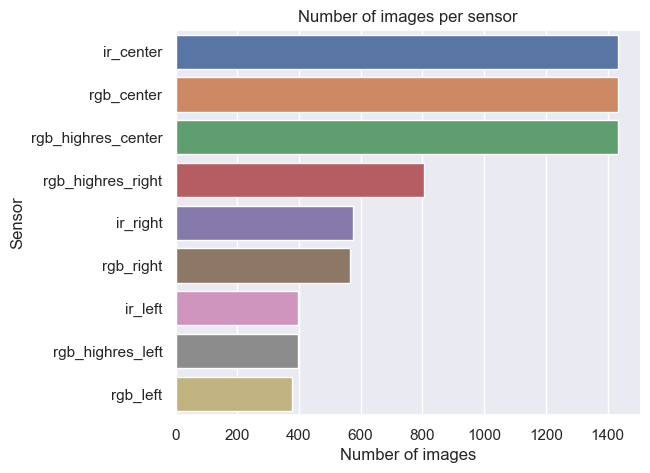
\includegraphics[width=0.9\textwidth]{images/datasets/db/images_per_sensor}
  \caption{Number of images per sensor.}
\end{subfigure}%
\begin{subfigure}[t]{.5\textwidth}
  \centering
  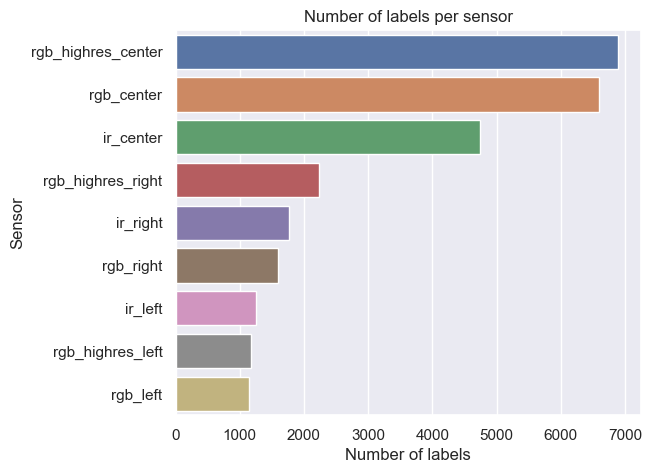
\includegraphics[width=0.9\textwidth]{images/datasets/db/labels_per_sensor}
  \caption{Number of labels per sensor}
\end{subfigure}
\caption{Number of images and labels per sensor, respectively.}
\label{fig:number_images}
\end{figure}


\begin{figure}[h]
\centering
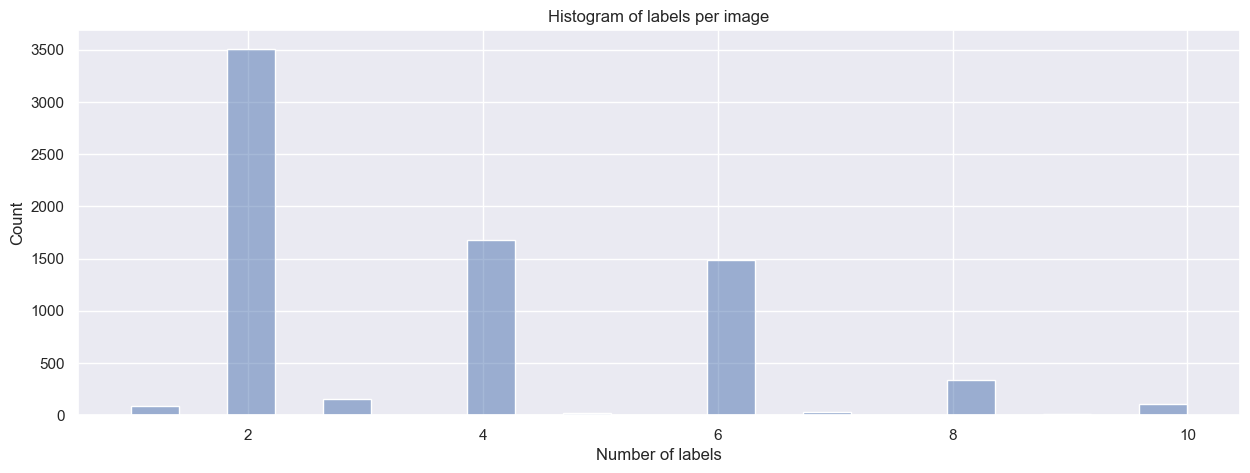
\includegraphics[width=0.9\textwidth]{images/datasets/db/labels_per_image}
\caption{Track labels per image. Most images depict track pairs. However, there are also images with odd number of tracks. }
\label{fig:labels_per_image}
\end{figure}

\begin{table}[h!]
\begin{center}
\begin{tabular}{|c| c c c|} 
  \hline
 Sensor &	Widht [px] &	Height [px] &	Aspect ration \\
 \hline
RGB low resolution &	4112 &	2504 &	1.64 \\
 \hline
RGB high resolution &	2464 &	1600 &	1.54 \\
 \hline
Infrared	& 640 &	480 &	1.33 \\
 \hline
\end{tabular}
\caption{Size of images per sensor.}
\label{tab:1}
\end{center}
\end{table}


All images were taken between 8AM and 17PM, so we cannot expect to test the effect of different sensors in the night. In particular, the RGB cameras fail to capture clear and detailed images in low-light conditions. 
Infrared cameras on the other hand, detect infrared radiation emitted by objects based on their temperature rather than visible light and are used in low-light conditions or complete darkness\footnote{All objects with a temperature greater than absolute zero emit infrared energy.}. The thermal radiation is converted into electrical signals which are then processed to a visual image that is visible to the human eye \citep{CLARK200283}. Warmer areas are displayed as brighter shades of gray while cooler areas appear as darker shades of gray.

Emissivity, a material property that indicates how efficiently an object emits infrared radiation, plays a significant role in thermal imaging. Emissivity is measured on a scale from 0 to 1, where 0 indicates a perfect reflection of the radiation (no emission such as a mirror), and 1 indicates perfect emissivity (total emission in an object referred to as blackbody).  Detecting rail tracks in infrared images is based on the principle that polished metallic surfaces such as tracks have a low emissivity, whereas organic materials that appear often in the background have a high emissivity.  


\subsection{Brightness of the images}


In deep learning, the quality of the images can have a large impact on the efficiency. In image segmentation tasks, where the goal is to identify and classify each pixel in an image, are particularly sensitive to variations in pixel brightness and intensity.
In this section, we analyze the brightness of the images for each type of sensor. Brightness is defined as the average pixel intensity $\frac{1}{N} \sum_{i=1}^{N} I_i $ ($N$ is the number of pixels in the image and $I_i$ is the intensity of pixel $i$). Figure~\ref{fig:brightness} shows a series of box plots with brightness values per sensor.


\begin{figure}[h]
\centering
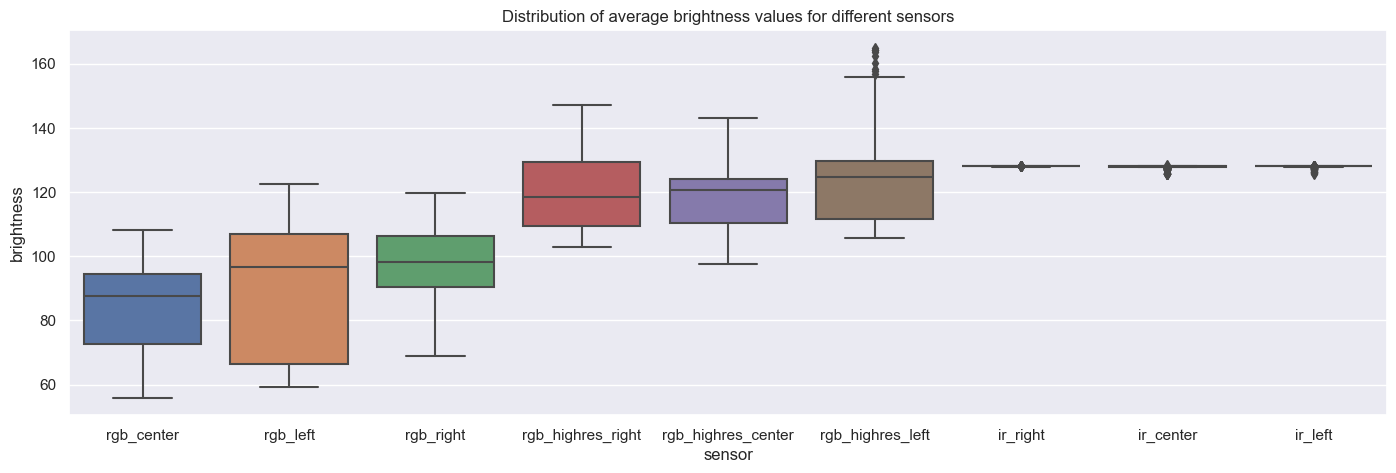
\includegraphics[width=0.9\textwidth]{images/datasets/db/brightness}
\caption{Brightness of images by sensor. }
\label{fig:brightness}
\end{figure}


Among the three types of sensors, low resolution RGB cameras produce the darkest images (a black image has a value of 0, a white image has a value of 255). 
High resolution images are brighter on average, which can be explained by different exposure settings such as shutter speed and ISO sensitivity. Both low and high-resolution cameras feature pixels of equal size ($3.45 \mu m$), so the amount of light per pixel is the same.
Infrared cameras produce images with almost constant brightness as the non-visible infrared image is mapped on a visible spectrum.

Figure~\ref{fig:brightness_examples} show one example of a bright and a dark image, respectively.


\begin{figure}
\centering
\begin{subfigure}[t]{.5\textwidth}
  \centering
  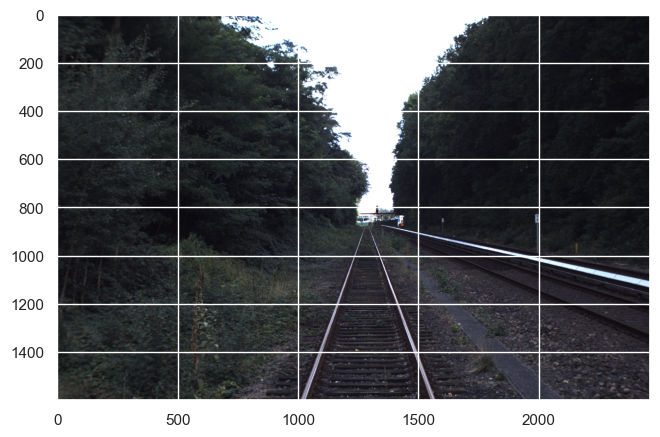
\includegraphics[width=0.9\textwidth]{images/datasets/db/dark}
  \caption{Image with low brightness value.}
%  \label{fig:sub1}
\end{subfigure}%
\begin{subfigure}[t]{.5\textwidth}
  \centering
  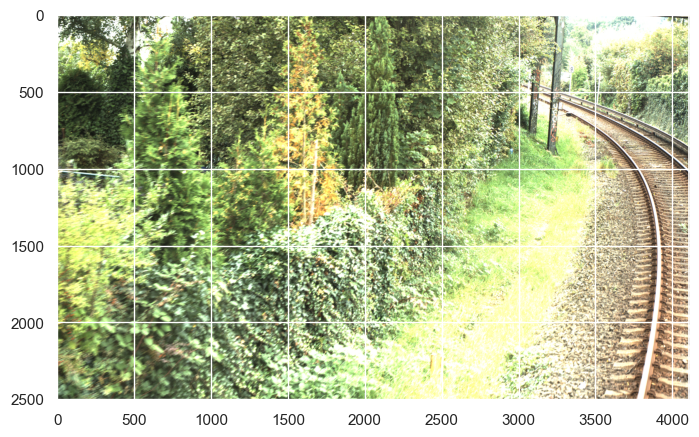
\includegraphics[width=0.9\textwidth]{images/datasets/db/bright}
  \caption{Image with high brightness value.}
 % \label{fig:sub2}
\end{subfigure}
\caption{Examples of very bright and very dark image, respectively.}
\label{fig:brightness_examples}
\end{figure}



\subsection{Entropy of the images} \label{sec:entropy}


Shannon entropy is a measure from information theory that reflects the uncertainty or randomness associated with a set of data \citep{6773024}. In the context of images, Shannon entropy can be used to quantify the complexity in the pixel values of an image. A high entropy value indicates higher complexity or randomness in the pixel values, while a low entropy value suggests more homogeneity. \cite{rahane2020measures} report a positive correlation between the entropy of the training data and the performance of semantic segmentation tasks, highlighting that more complex images are harder to learn by deep-learning networks.
The Shannon entropy for a grayscale image is given by $H(X) = -\sum_{i=1}^{n} P(x_i) \cdot \log_2(P(x_i))$, where $P(x_i)$ is the probability of occurrence of pixel $x_i$ (i.e., the number of pixels with intensity $x_i$ divided by the total number of pixels). 
A box-plot with the entropy distribution is given in Figure~\ref{fig:entropy} for each sensor. The maximum entropy value is $8 = \log_2(256)$ as we convert the images to grayscale with 256 different intensity levels.


\begin{figure}[h]
\centering
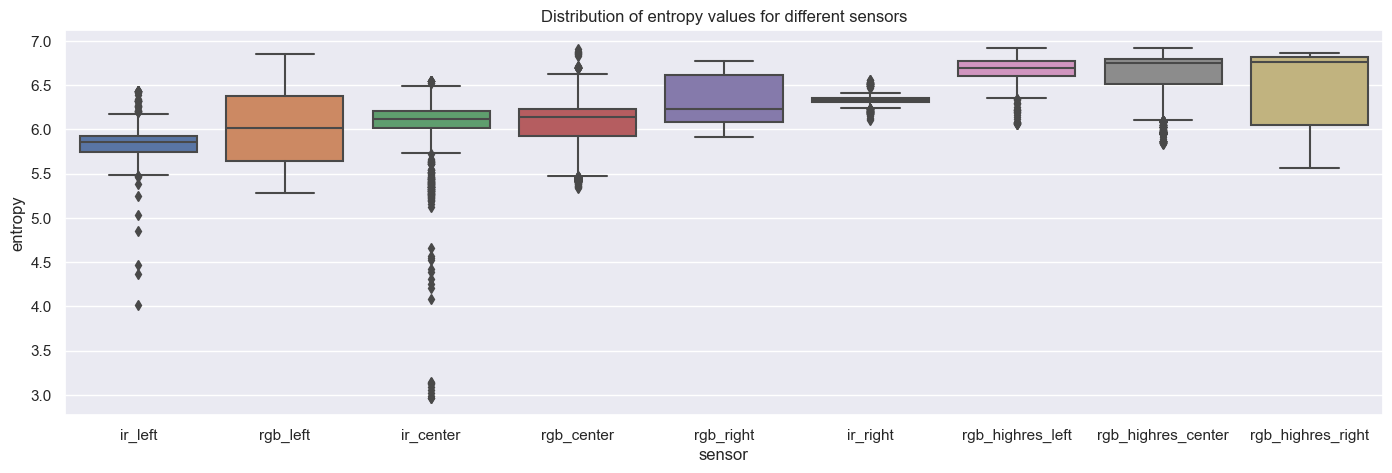
\includegraphics[width=0.9\textwidth]{images/datasets/db/entropy}
\caption{Entropy of images by sensor. }
\label{fig:entropy}
\end{figure}

Overall, the images have a high entropy -- the median values range from 5.9 to 6.8. High resolution images have the highest entropy. Infrared images do not seem to have lower entropy on average. However, certain images have a very low randomness and as it turns out also very low level of information when looking at Figure~\ref{fig:entropy_sub1}. Figure~\ref{fig:entropy_examples} highlight the visual difference between a very low and a very high entropy image.





\begin{figure}
\centering
\begin{subfigure}[t]{.5\textwidth}
  \centering
  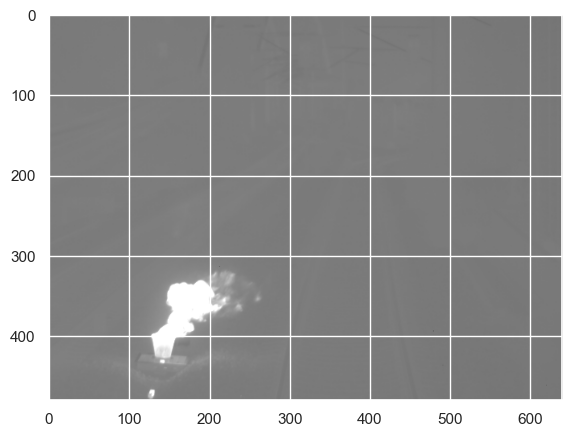
\includegraphics[width=0.9\textwidth]{images/datasets/db/low_entropy}
  \caption{Image with low entropy value.}
  \label{fig:entropy_sub1}
\end{subfigure}%
\begin{subfigure}[t]{.5\textwidth}
  \centering
  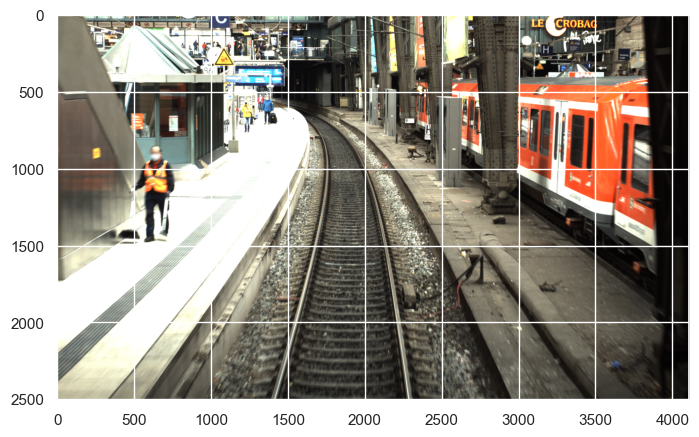
\includegraphics[width=0.9\textwidth]{images/datasets/db/high_entropy}
  \caption{Image with high entropy value.}
 \label{fig:entropy_sub2}
\end{subfigure}
\caption{Examples of image with minimal and maximal entropy, respectively.}
\label{fig:entropy_examples}
\end{figure}


\subsection{Occlusion}

Certain track labels are hidden or occluded by other objects. One example is given in Figure~\ref{fig:entropy_sub2} where the train on the right covers the tracks.
In this section, we analyze the occlusion of the labels and examine those occlusions visually.

Figure~\ref{fig:occul_hist} shows the number of labels with a given occlusion level. Most of the labels, 20.069, are not occluded at all or have only a slight occlusion. However, 320 labels in 196 images are marked with an occlusion level of 100\%. Figure~\ref{fig:occlusion_examples} shows two examples where the track labels are fully covered.


\begin{figure}[h]
\centering
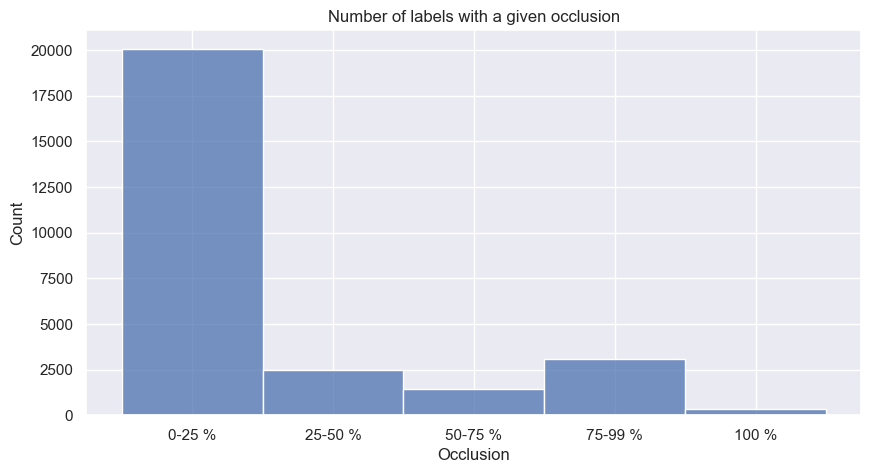
\includegraphics[width=0.9\textwidth]{images/datasets/db/occlusion_hist}
\caption{Histogram showing the occlusion level for track labels. }
\label{fig:occul_hist}
\end{figure}



We keep all images in the dataset as the CNN might recognize that there has to be a track below a train and because most images with covered labels contain visible labels as well.


\begin{figure}
\centering
\begin{subfigure}[t]{.5\textwidth}
  \centering
  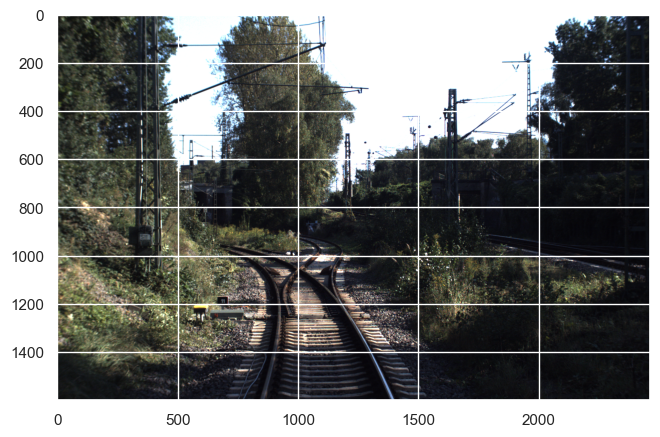
\includegraphics[width=0.9\textwidth]{images/datasets/db/occlusion_example1}
  \caption{Track on the right is hard to recognize due to poor lighting condition.}
\end{subfigure}%
\begin{subfigure}[t]{.5\textwidth}
  \centering
  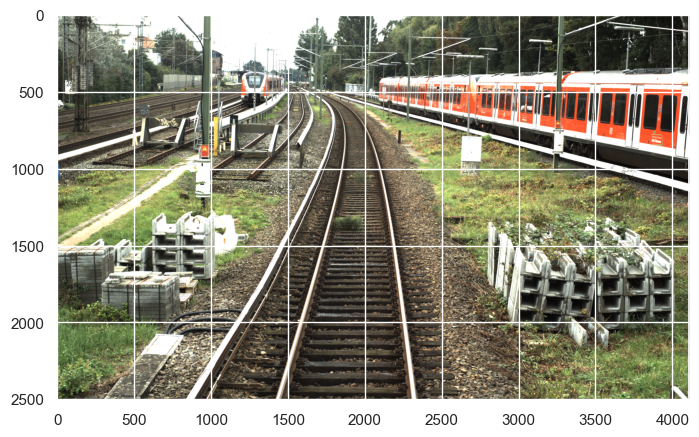
\includegraphics[width=0.9\textwidth]{images/datasets/db/occlusion_example2}
  \caption{Track is covered by train \\ on the right. }
\end{subfigure}
\caption{Examples of track labels with 100\% occlusion.}
\label{fig:occlusion_examples}
\end{figure}


\subsection{Images and video frames}

The rail tracking systems aim to analyze video streams by treating each video frame as an independent image. Consequently, the images in the OSDaR23 dataset represent individual frames extracted from video sequences. 	Figure~\ref{fig:video} shows three examples of video sequences with seven frames each. It is clear that there is only minor variation in the images.


\begin{figure}
\centering
\begin{subfigure}[t]{\textwidth}
  \centering
  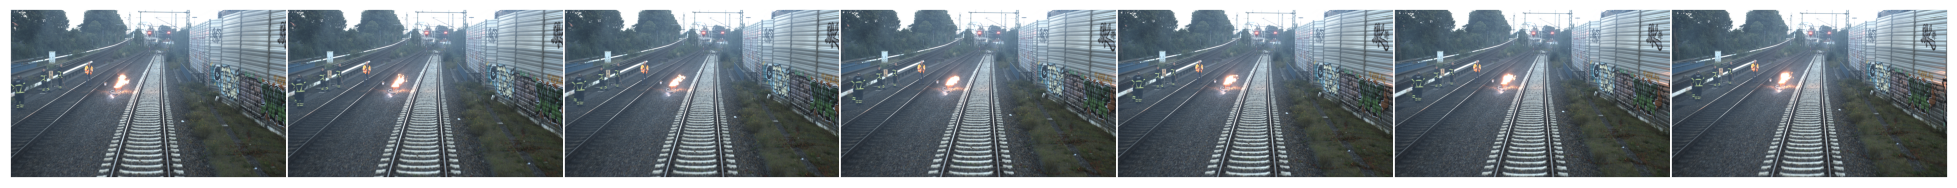
\includegraphics[width=0.9\textwidth]{images/datasets/db/video_1}
\end{subfigure}%
\vskip\baselineskip
\begin{subfigure}[t]{\textwidth}
  \centering
  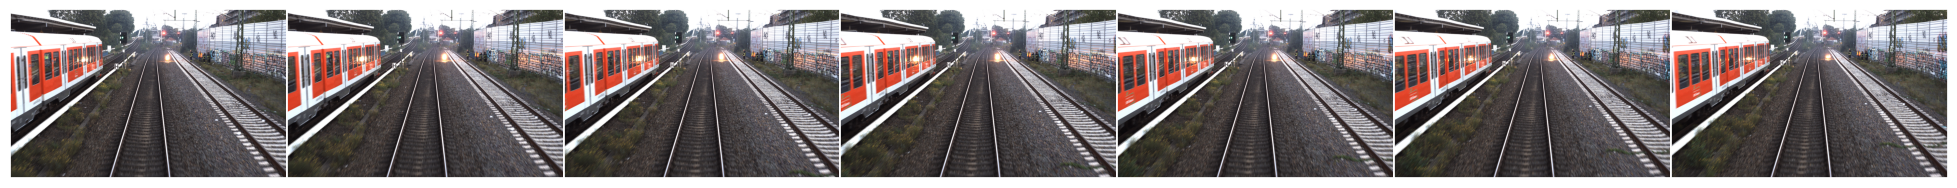
\includegraphics[width=0.9\textwidth]{images/datasets/db/video_2}
\end{subfigure}
\vskip\baselineskip
\begin{subfigure}[t]{\textwidth}
  \centering
  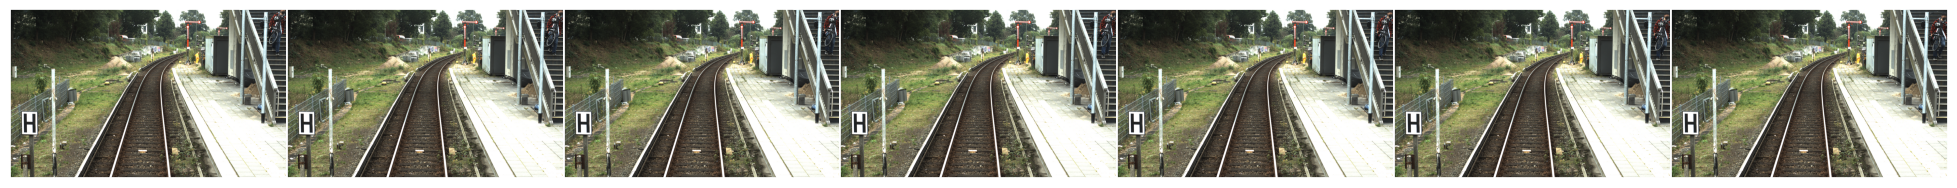
\includegraphics[width=0.9\textwidth]{images/datasets/db/video_3}
  \label{fig:sub3}
\end{subfigure}
\caption{Three examples with seven video frames (i.e., images), respectively.}
\label{fig:video}
\end{figure}


Two major issues when training a model on a dataset that consists of similar images is a lack of generalization (i.e., inability to generalize well on diverse and unseen images) and reduced robustness (i.e., vulnerability to variations in lighting conditions and backgrounds). 
In order to mitigate the issues, we add images from the RailSem19 dataset to the training data.




\section{RailSem19 dataset}

The RailSem19 dataset \citep{9025646} is not the primary focus of this thesis. However, the previous analysis reveals that among the 7.421 images within the OSDaR23 dataset, a significant number show high similarity. This similarity is due to the fact that the images are frames from a video sequence and the presence of three cameras for each orientation.
The RailSem19 dataset is added to the training set in order to increase the performance of the segmentation approach.
In the following, we will examine the RailSem19 dataset in more detail.

The dataset consists of 8500 rail images taken in different countries, and weather and lighting conditions. The number of rail annotations is 58.483. All images have a size of 1920x1080 pixels. 
Figure~\ref{fig:labels_per_image_railsem} shows a histogram of images with the respective number of track labels on a log scale. Most images contain 4 track labels (i.e., two pairs of tracks) but the dataset also contains complicated networks with 26 pairs of tracks. An example of a simple and an example of a complicated infrastructure is given in Figure~\ref{fig:railsem_complicated_vs_simple}.



\begin{figure}[h]
\centering
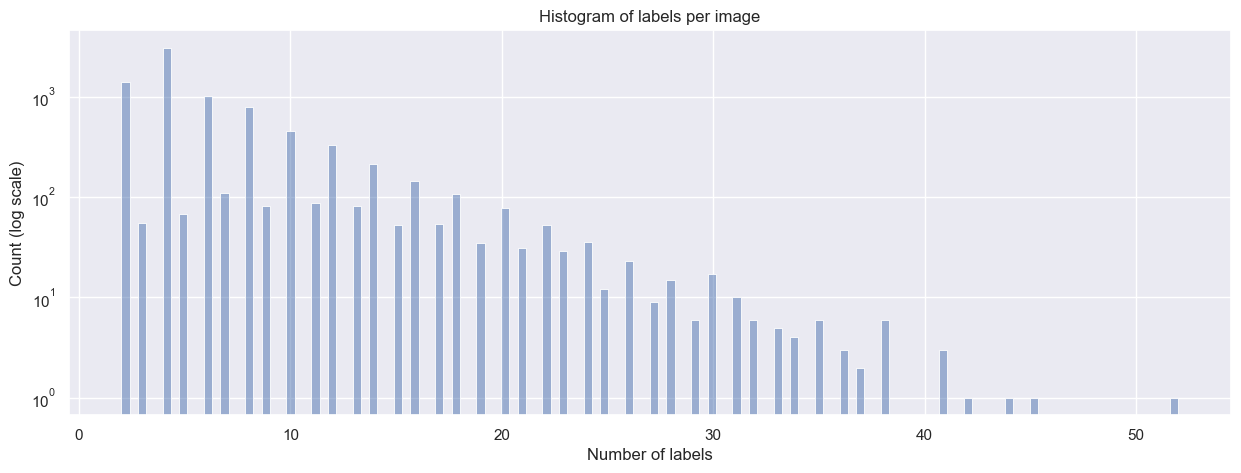
\includegraphics[width=0.9\textwidth]{images/datasets/railsem/labels_per_image}
\caption{Track labels per image on a logarithmic scale. The images range from simple railroads with a single pair of tracks to complicated networks with 26 pairs of tracks. }
\label{fig:labels_per_image_railsem}
\end{figure}


\begin{figure}
\centering
\begin{subfigure}[t]{.5\textwidth}
  \centering
  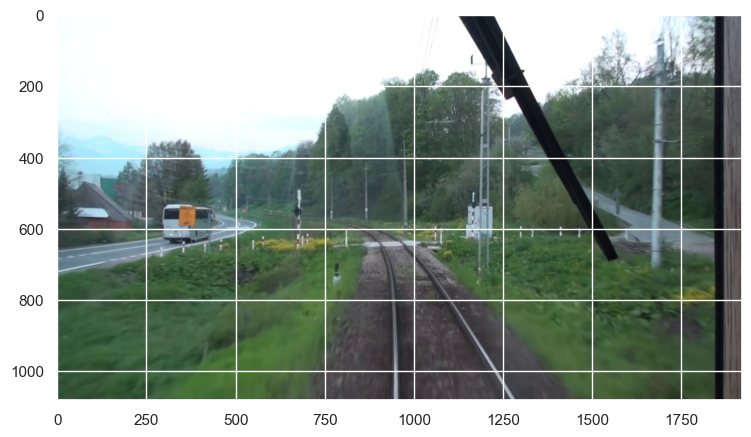
\includegraphics[width=0.9\textwidth]{images/datasets/railsem/example_2_tracks}
  \caption{Simple rail infrastructure.}
\end{subfigure}%
\begin{subfigure}[t]{.5\textwidth}
  \centering
  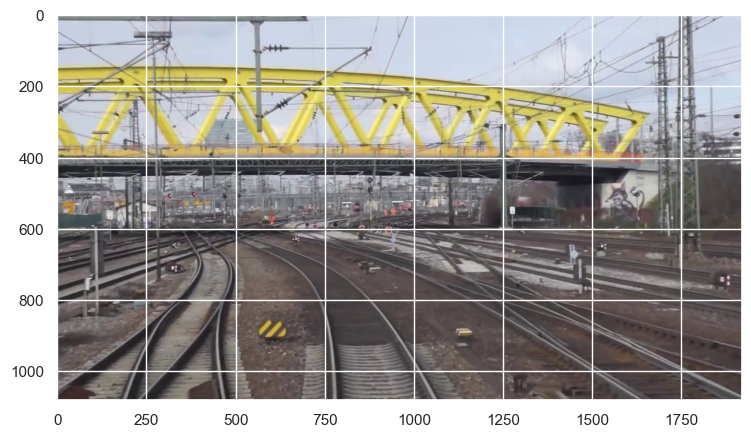
\includegraphics[width=0.9\textwidth]{images/datasets/railsem/example_52_tracks}
  \caption{Complicated rail infrastructure. }
\end{subfigure}
\caption{Examples of simple and complicated rail infrastructure.}
\label{fig:railsem_complicated_vs_simple}
\end{figure}


Figure~\ref{fig:railsem_brightness} and  Figure~\ref{fig:railsem_entropy} show the distribution of the brightness values and the entropy values as defined in Section~\ref{sec:OSDaR23}, respectively. The RailSem19 images are mostly brighter than the OSDaR23; the distribution of the values ranges from almost black images to almost white images (see Figure~\ref{fig:railsem_sub1} and Figure~\ref{fig:railsem_sub2}). The entropy of the RailSem19 images is similar to the images in the OSDaR23 dataset. The outliers at the lower end of the entropy spectrum are associated with infrared images in the OSDaR23 dataset. However, in RailSem19 low entropy images are often images that were generated in tunnels or at night. Figure~\ref{fig:railsem_sub2} and Figure~\ref{fig:railsem_sub4} are images with a low entropy levels close to zero whereas Figure~\ref{fig:railsem_sub3} has the highest entropy level in the data set with a score of 6.97.


\begin{figure}
\centering
\begin{subfigure}[t]{.5\textwidth}
  \centering
  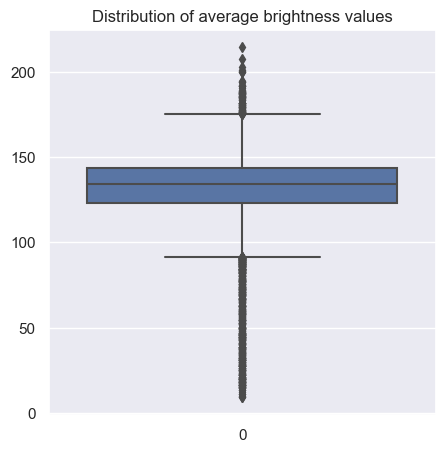
\includegraphics[width=0.9\textwidth]{images/datasets/railsem/brightness}
  \caption{Boxplot of brightness values.}
   \label{fig:railsem_brightness}
\end{subfigure}%
\begin{subfigure}[t]{.5\textwidth}
  \centering
  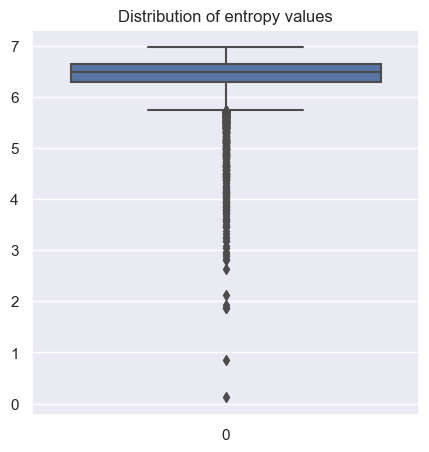
\includegraphics[width=0.9\textwidth]{images/datasets/railsem/entropy}
  \caption{Boxplot of entropy values. }
  \label{fig:railsem_entropy}
\end{subfigure}
\caption{Brightness and entropy of RailSem19 images.}
\label{fig:railsem_brightness_entropy}
\end{figure}




\begin{figure}
\centering
\begin{subfigure}[t]{.5\textwidth}
  \centering
  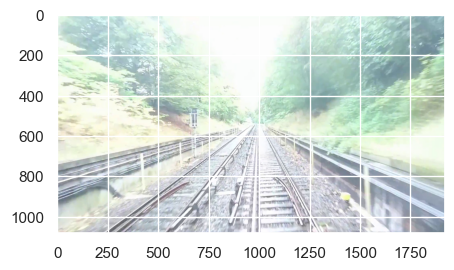
\includegraphics[width=0.9\textwidth]{images/datasets/railsem/example_bright}
  \caption{Bright image.}
  \label{fig:railsem_sub1}
\end{subfigure}%
\begin{subfigure}[t]{.5\textwidth}
  \centering
  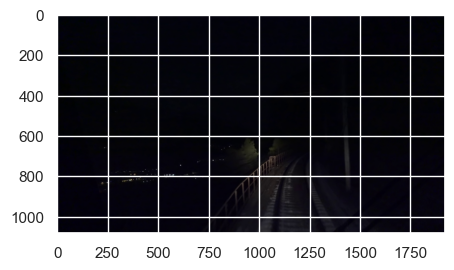
\includegraphics[width=0.9\textwidth]{images/datasets/railsem/example_dark}
  \caption{Dark image.}
  \label{railsem_sub2}
\end{subfigure}
\vskip\baselineskip
\begin{subfigure}[t]{.5\textwidth}
  \centering
  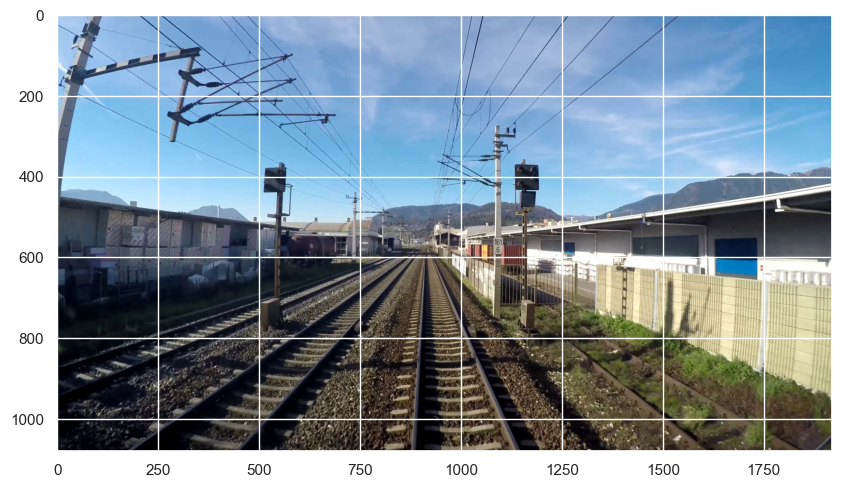
\includegraphics[width=0.9\textwidth]{images/datasets/railsem/example_high_entropy}
  \caption{High entropy.}
  \label{railsem_sub3}
\end{subfigure}%
\begin{subfigure}[t]{.5\textwidth}
  \centering
  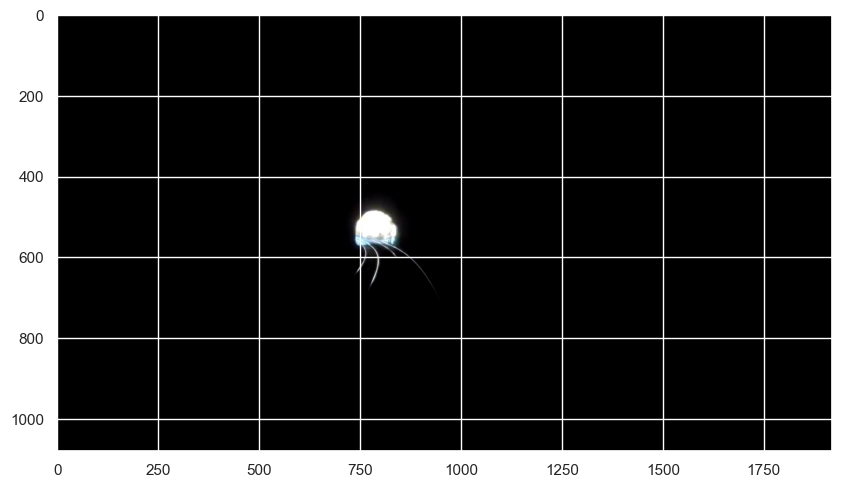
\includegraphics[width=0.9\textwidth]{images/datasets/railsem/example_low_entropy}
  \caption{Low entropy.}
  \label{railsem_sub4}
\end{subfigure}
\caption{Extreme examples with regard to brightness and entropy.}
\label{fig:examples}
\end{figure}


\section{Data splitting}

Splitting a dataset into training, validation, and test sets is a standard practice in machine learning to evaluate and improve the performance of a model. 
 Separating data into distinct sets and using them at different stages of development prevents unintended data leakage where information from the test or validation set influences the training process.
 
%The validation set assesses performance during training, refines hyperparameters, and guards against overfitting. Adjustments made based on validation set evaluations ensure the model generalizes effectively to new, unseen data. 

The training set is used to train the model -- the model learns patterns and relationships within the training data.
The validation set is used to evaluate the performance during the training process, fine-tune the hyperparameters of the model, and to prevent overfitting (i.e., a situation when a model performs well on the training data but fails to generalize to new data). Adjustments to the algorithm without compromising the model's ability to generalize to new data can be made by evaluating the performance on the validation set. 
The test set is reserved for the final evaluation of the model. The test set allows for an unbiased assessment of the model's performance on data it has never seen before and provides, therefore, an estimate of how well the model is likely to perform in real-world applications.

We perform a random split with a share of 70\%/15\%/15\% for train, validation, and test set respectively. Splitting the RailSem19 set is straightforward; we randomly assign images to each set resulting in 5.950, 1.275, and 1.275 images per set, respectively. However, the OSDaR23 comprises many images that are very similar (e.g., frames from a video that were taken when the locomotive was standing still), so we perform a random split not on individual images but on videos sequences. The approach results in 5.506 images for training, 987 images for validation, and 928 images for testing.
The assignment of video sequences to the respective set and the split on sensor level is given in Appendix~\ref{app:data_split}



\chapter{Solution approach and experiments} % 4000 words

Given an image captured by an on-board camera on the locomotive, our objective is to precisely segment the visible rail tracks. %The output is  a polyline describing each track.

Within computer vision, semantic segmentation is a well-studied domain focusing on classifying each pixel in an image into predefined categories \citep{MO2022626}. Conceptually, it 
can be seen as an extension of object detection, a technique that recognizes and precisely locates objects within an image using bounding boxes.
The pixel-level precision in object classification enables the understanding of the image context and is therefore often used in applications like autonomous driving and robotics.

%Our approach to the rail detection problem is based on two steps. First, we perform a semantic segmentation where each pixel is classified as either rail track or background. 
%In a second step, the result of the segmentation task is used to define one polyline for each track.
 The segmentation is performed by the YOLOv8 algorithm \citep{Jocher_Ultralytics_YOLO_2023}.  YOLOv8, short for "You Only Look Once, version 8," is the latest version in the YOLO series of real-time object detectors, offering state-of-the-art performance in terms of accuracy and speed \citep{ultralytics_docs}. YOLOv8 builds upon the YOLO architecture, introduced in \cite{redmon2016you} -- a paper that has received more than 43.000 citations at the time of writing. Since the introduction of the original YOLO in 2016, the framework has been tested extensively with remarkable results (e.g., \cite{JIANG20221066, cryptography6020016, Diwan2023}). The efficiency of the YOLO implementations by \cite{Jocher_Ultralytics_YOLO_2023} for segmentation tasks is examined in \cite{agriculture13081643} and \cite{STRAKER2023100045}.


\cite{meyer2021yolino} introduce YOLinO, a versatile and efficient algorithm inspired by YOLO. It is designed to detect polylines in the context of lane detection, as discussed in Section~\ref{sec:lane_detection}. While the proposed approach is suitable for rail track detection, adapting the existing code base from lane detection to rail track detection exceeds the scope of this thesis. Furthermore, our goal is to employ an off-the-shelf solution framework that can be readily utilized by a broader audience.

In order to evaluate the YOLOv8 approach, we devise a track detection algorithm based on the fast line detector (FLD) by \cite{FLD}.
In the following, we describe the YOLOv8 and the FLD approach, and give details of the infrastructure for running the experiments.

\section{Infrastructure}

Experiments are run on the High Performance Lab Cluster (HPL) of the UAS Technikum Wien. 
The HPL comprises 19 PCs connected through a 10-GBit-Network. The PCs have the following setup, respectively: AMD Ryzen 9 3900X 12-Core Processor, NVIDIA GeForce RTX 2080 Ti GPU, 32 GB RAM, and 80 GB Hard Disk.

All nodes are running Linux Ubuntu 20. CUDA libraries are installed for GPU management. All scripts we written in Python 3.8.10. 


\section{Transforming labels} 

In semantic segmentation, labels are often represented as closed polygons. Each polygon corresponds to a specific semantic class and the pixels enclosed within the polygon are assigned the label of that class.
However, the track labels in both OSDaR23 and RailSem19 dataset are given as polylines. Therefore, we transform the labels as follows. First, we adjust the thickness of the polyline such that is covers the tracks. Second, we generate the mask -- a binary image where each pixel is assigned a value indicating the category it belongs to (i.e., track or background). Finally, the boundaries of the track label are extracted by using the $drawContours$ and $approxPolyDP$ functions in the OpenCV library. The vectors defining the polygons are written to disk and are loaded during the training.  Figure~\ref{fig:labeling} illustrates the transformation process.


\begin{figure}
\centering
\begin{subfigure}[t]{.5\textwidth}
  \centering
  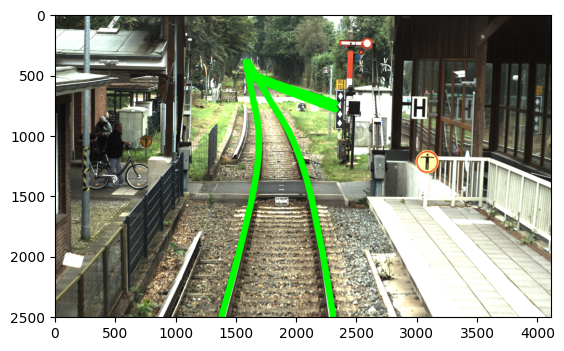
\includegraphics[width=0.9\textwidth]{images/labeling/polylines}
  \caption{Estimate thickness such that the lines \\ cover the tracks.}
 % \label{fig:railsem_sub1}
\end{subfigure}%
\begin{subfigure}[t]{.5\textwidth}
  \centering
  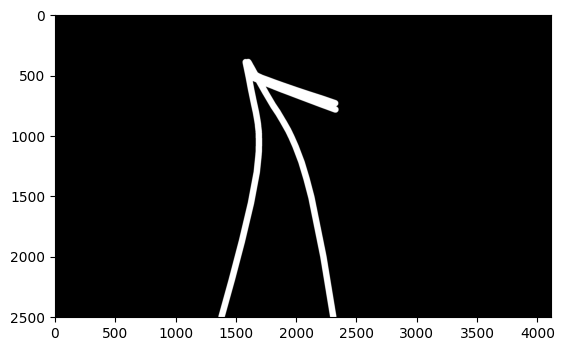
\includegraphics[width=0.9\textwidth]{images/labeling/mask}
  \caption{Create mask (i.e., binary mapping of track labels and background).}
%  \label{railsem_sub2}
\end{subfigure}
\vskip\baselineskip
\begin{subfigure}[t]{.5\textwidth}
  \centering
  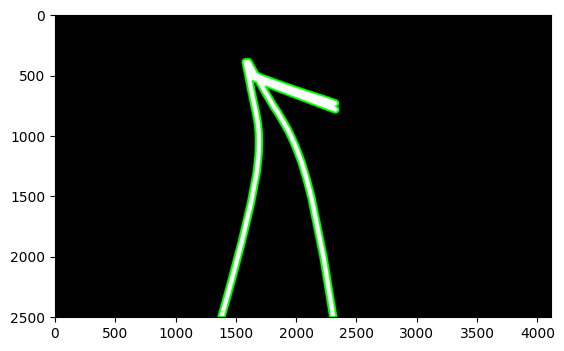
\includegraphics[width=0.9\textwidth]{images/labeling/contour}
  \caption{Extract contour of track label (see green boundary in mask).}
%  \label{railsem_sub3}
\end{subfigure}%
\begin{subfigure}[t]{.5\textwidth}
  \centering
  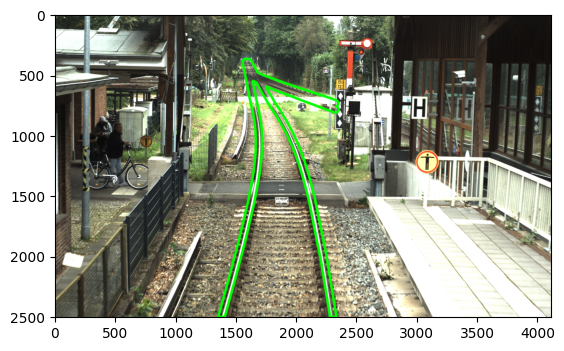
\includegraphics[width=0.9\textwidth]{images/labeling/final}
  \caption{Polygon is enclosing the \\ region of interest.}
%  \label{railsem_sub4}
\end{subfigure}
\caption{Process of transforming the labels from  polyline to polygon.}
\label{fig:labeling}
\end{figure}


The presented approach generates polygons based on the segmentation mask. In order to test the effect of the labeling strategy, we also generate labels for each rail track separately. Figure~\ref{fig:labeling2} illustrates the difference between the two labeling approaches. The unified polygon base on the mask is shown on the left; on the right, each track is labeled separately.



\begin{figure}
\centering
\begin{subfigure}[t]{.5\textwidth}
  \centering
  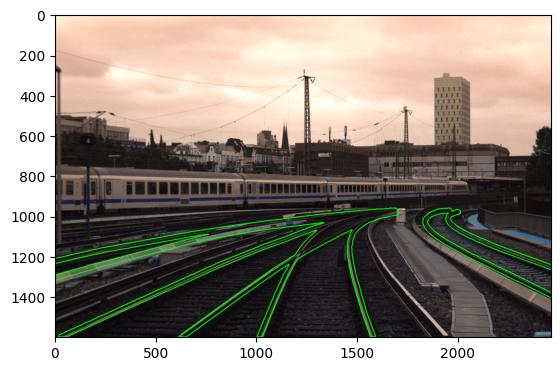
\includegraphics[width=0.9\textwidth]{images/labeling/label_union}
  \caption{All tracks are labeled by two closed polygons.}
 % \label{fig:railsem_sub1}
\end{subfigure}%
\begin{subfigure}[t]{.5\textwidth}
  \centering
  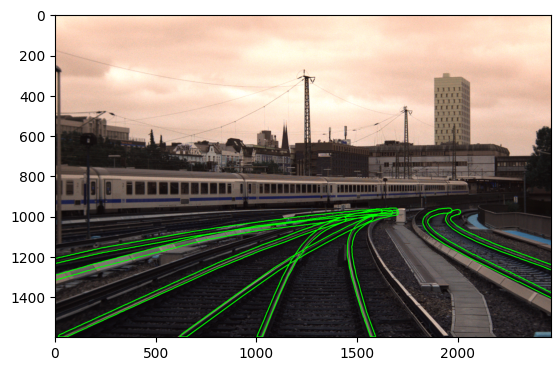
\includegraphics[width=0.9\textwidth]{images/labeling/label_single}
  \caption{Each track is labeled by a separate polygon.}
%  \label{railsem_sub2}
\end{subfigure}
\caption{Two different approaches for labeling tracks.}
\label{fig:labeling2}
\end{figure}



\section{Performance evaluation}

There is a number of performance metrics that are typically used in semantic segmentation to evaluate the effectiveness of the models \citep{Taha2015}. The choice of metrics depends on the specific requirements of the application and the nature of the dataset. In this section, we will introduce and examine different metrics for the rail segmentation task. \\


\noindent\textbf{Pixel Accuracy} provides a simple measure of the overall accuracy by considering correctly predicted pixels. 


\[
\text{Pixel Accuracy} = \frac{\text{Number of Correctly Predicted Pixels}}{\text{Total Number of Pixels}}
\]

\vspace{1cm}

\noindent\textbf{Precision} measures the accuracy of positive predictions among all positive predictions. The metric is important when minimizing false positives is critical (e.g., in medical diagnostics).

\[
\text{Precision} = \frac{\text{TP}}{\text{TP} + \text{FP}}
\]
True Positives (TP) are the instances where the model correctly predicts the positive class (i.e., it correctly identifies the track).
False Positives (FP) are the instances where the model incorrectly predicts the positive class (i.e., it identifies a track when it is actually absent). \\

\vspace{1cm}

\noindent\textbf{Recall} measures the ability to capture all positive instances. Recall is optimized when it is crucial to identify all instances of a particular class, even at the cost of some false positives.

\[
\text{Recall} = \frac{\text{TP}}{\text{TP} + \text{FN}}
\]
False Negatives are the instances where the model incorrectly predicts the negative class (i.e., it identifies background even when the there is a track). \\

\vspace{1cm}

\noindent\textbf{Dice score or F1 score} balances precision and recall which is particularly useful when dealing with unbalanced datasets, i.e., when one class has a much larger or smaller number of pixels compared to the other class (in our case background vs. tracks). Dice and F1 score are the most used metrics in segmentation when the dataset is unbalanced. Some authors use the Dice score while others use the F1 score with the respective formulas given below. However, it can be shown that one reduces to the other. 


\[
\text{Dice Score} = \frac{2 \times \text{TP}}{2 \times \text{TP} + \text{FP} + \text{FN}}
\]

\begin{align*}
    \text{F1 Score} &= \frac{2 \times \text{Precision} \times \text{Recall}}{\text{Precision} + \text{Recall}} \\
    \vspace{1em}
     &= \frac{2 \cdot \frac{\text{TP}}{\text{TP} + \text{FP}} \cdot \frac{\text{TP}}{\text{TP} + \text{FN}}}{\frac{\text{TP}}{\text{TP} + \text{FP}} + \frac{\text{TP}}{\text{TP} + \text{FN}}} \\
    \vspace{1em}
     &= \frac{2 \cdot \text{TP}}{2 \cdot \text{TP} + \text{FP} + \text{FN}}
\end{align*}


\vspace{1cm}

\noindent\textbf{Intersection over Union (IoU) or Jaccard index}, measures the overlap between predicted and ground truth regions. The metric is commonly used to evaluate the spatial accuracy of segmentation masks. Apart from the boundary values \{0,1\}, the IoU score is consistently smaller than the Dice score.

\[
\text{IoU} = \frac{\text{TP}}{\text{TP} + \text{FP} + \text{FN}}
\]

\vspace{1cm}

In Figure~\ref{fig:example_metrcis}, we illustrate the performance metrics based on an example. Figure~\ref{fig:gt_sub1} shows the ground truth label, i.e., the correct mask of the image being analyzed. Figure~\ref{fig:ex_sub1} shows five possible predictions, where Image~5 is simply a black image with no positive classifications. The metrics for the five predictions are given in Figure~\ref{tab:metrics}. The example shows that Pixel accuracy is not appropriate in unbalanced dataset -- even Image 5 which has no prediction at all has an accuracy score of almost 95\%. Image 2 yields a high Precision score of 0.706 as the FN values are not accounted for.  Recall seems to be a strong predictor of performance in this example. However, an all white image (i.e., all pixels classified as track) would yield a perfect Recall. Dice and IoU are best suited to distinguish between good and bad predictions. Both values have a wide range and the scores are in line with the estimation based on visual inspection.

Based on the literature and the example, we choose the Dice score to analyze the performance of different models.

\begin{figure}
\centering
\begin{subfigure}[t]{.9\textwidth}
  \centering
  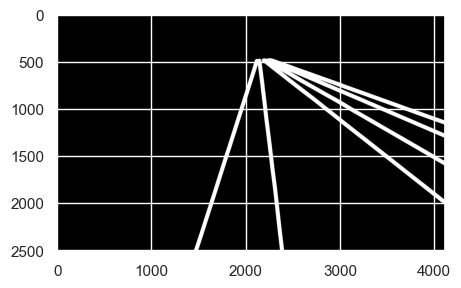
\includegraphics[width=0.5\textwidth]{images/performance/ground_truth}
  \caption{Ground truth label selected randomly from training set.}
   \label{fig:gt_sub1}
\end{subfigure}%
\vskip\baselineskip
\begin{subfigure}[t]{0.9\textwidth}
  \centering
  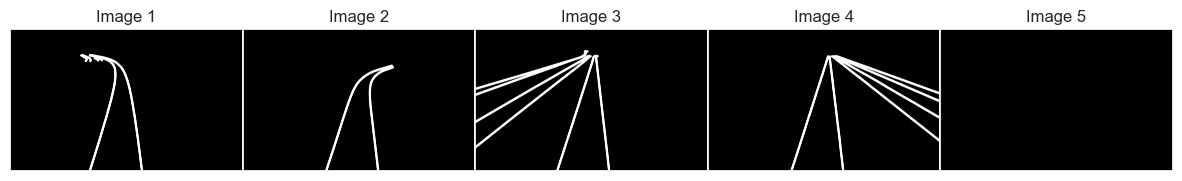
\includegraphics[width=\textwidth]{images/performance/examples}
  \caption{Example predictions selected randomly from training set; last image is only background illustrating a case where no rail track was found.}
\label{fig:ex_sub1}
\end{subfigure}
\vskip\baselineskip
\begin{subfigure}[t]{0.9\textwidth}
  \centering
    \footnotesize
  \begin{tabular}{|c|ccccc|}
       \hline
      Image & Pixel Accuracy & Precision & Recall & Dice & IoU \\
      \hline
      1 & 0.927 & 0.013 & 0.005 & 0.007 & 0.004 \\
      2 & 0.956 & 0.706 & 0.249 & 0.369 & 0.226 \\
      3 & 0.916 & 0.197 & 0.201 & 0.199 & 0.111 \\
      4 & 0.999 & 0.992 & 0.991 & 0.991 & 0.983 \\
      5 & 0.948 & -$^{\mathrm{a}}$ & 0.0 & 0.0 & 0.0 \\
       \hline
       \multicolumn{6}{l}{$^{\mathrm{a}}$Division by zero as there are no positive classifications.} \\
  \end{tabular}
  \caption{Performance Metrics.}
  \label{tab:metrics}
\end{subfigure}
\caption{Example masks -- ground truth vs. prediction.}
\label{fig:example_metrcis}
\end{figure}


\section{Non-AI based segmentation}

To assess the performance of the YOLO approach, we establish a baseline using a traditional line detection method. Specifically, we employ the fast line detection algorithm based on Hough transform, as implemented by \cite{FLD}. In a post-processing step, we incorporate domain specific knowledge to improve the results.
In this section, we describe the baselining approach in detail.
 
 \subsection{Fast line detection}


The fast line detection algorithm as proposed by \cite{fld_inproceedings} operates as follows: 
First, edges in the image are detected using a Canny edge detector. The system then extracts line segments by connecting edge pixels with straight lines and extending them until they satisfy the co-linearity conditions (i.e., whether or not the newly added pixels align well with the existing segment in terms of forming a straight line). Points that deviate from forming a straight line are considered endpoints of other segments. 

%First, edges in the image are detected using a Canny edge detector. The Hough transform is then applied in order to represent lines in a parameter space known as the Hough space. For each edge pixel (i.e., points where the intensity changes along a line), a set of potential lines in the Hough space is generated by varying slope and intercept. Each edge pixel effectively "votes" for the lines it might belong to in the Hough space. After the voting process, lines that receive a sufficient number of votes are considered potential lines in the image. Finally, the identified lines are extracted based on the parameters slope and intercept that receive more votes than a predefined threshold.
FLD is suitable for applications where speed is crucial such as real-time systems or applications where processing resources are limited.
The exact implementation details vary based on the specific version of OpenCV and underlying optimizations that are applied.

\subsection{Postprocessing}

The results of the FLD algorithm are post-processed to incorporate domain specific knowledge. More precisely, we filter out lines based on the observation that cameras with different orientations capture rail tracks that are bounded by boxes of different aspect ratios. Figure~\ref{fig:bb_examples} illustrate the idea: Figure~\ref{fig:bb_long} shows an image of a forward facing camera; the aspect ration of the bounding box enclosing the track is large.  Figure~\ref{fig:bb_wide} shows an image of a left facing camera; the aspect ratio of the bounding box enclosing the track is small.


\begin{figure}
\centering
\begin{subfigure}[t]{.5\textwidth}
  \centering
  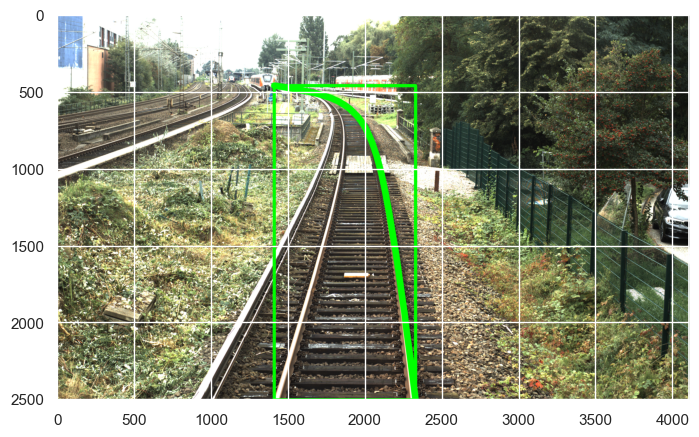
\includegraphics[width=0.9\textwidth]{images/datasets/db/aspect_ratio_long}
  \caption{Center camera: elongated bounding box aspect ratio.}
   \label{fig:bb_long}
\end{subfigure}%
\begin{subfigure}[t]{.5\textwidth}
  \centering
  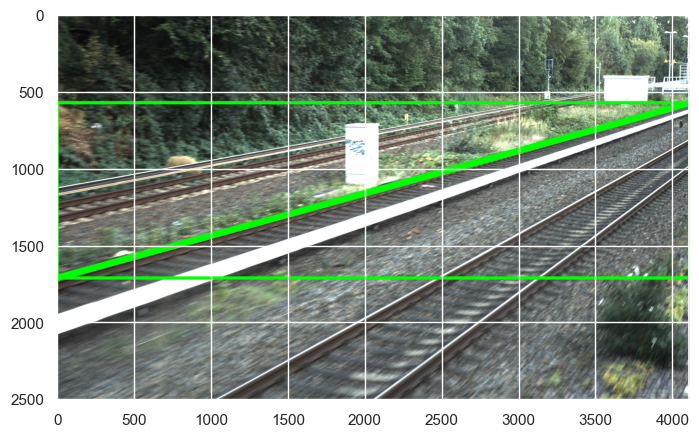
\includegraphics[width=0.9\textwidth]{images/datasets/db/aspect_ratio_wide}
  \caption{Left camera: wide bounding box \\ aspect ratio. }
  \label{fig:bb_wide}
\end{subfigure}
\caption{Different bounding box aspect ratios depending on camera orientation.}
\label{fig:bb_examples}
\end{figure}

Figure~\ref{fig:bb_aspect_ratio_hist} gives the distribution of the bounding box aspect ratios for the different camera orientations in the OSDaR23 dataset. 
The histogram confirms the idea that different sensors have different aspect ratios for the bounding boxes. For more details see Appendix~\ref{app:fld}.


\begin{figure}[h]
\centering
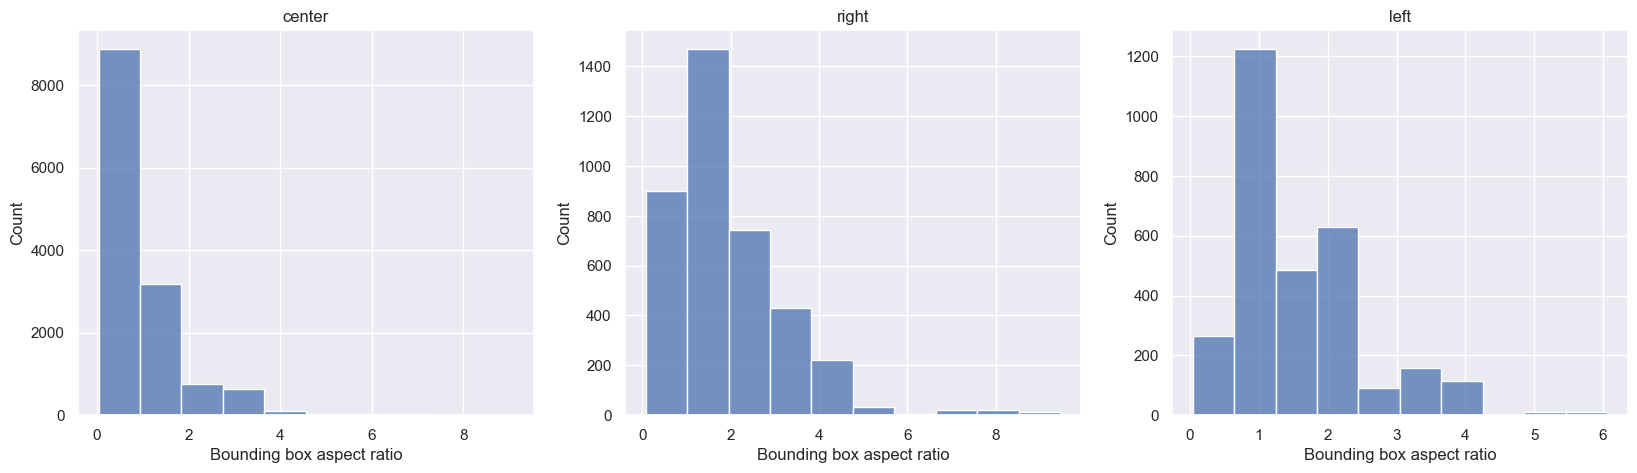
\includegraphics[width=0.9\textwidth]{images/datasets/db/bb_ascpect_ratio_hist}
\caption{Histogram of bounding box aspect ratios by camera orientation. }
\label{fig:bb_aspect_ratio_hist}
\end{figure}

The aspect ratios are used to remove all lines detected by FLD that have a bounding box aspect ratio smaller than the $x^{th}$ quantile or larger than the $1-x^{th}$ quantile.

In a final step, we apply Connected Component Labeling (CCL) to remove noise or segments that are false positives \citep{CCL}. 
The goals of CCL is to identify and label connected regions in a binary image where pixels are either tracks or background. After connected components are labeled in the image, we remove all components that are x\% smaller than the largest component.

The entire process is illustrated in Figure~\ref{fig:fld_demo}. The final result showcases that the approach is a heuristic that might filter out true positive labels.

\begin{figure}[h]
\centering
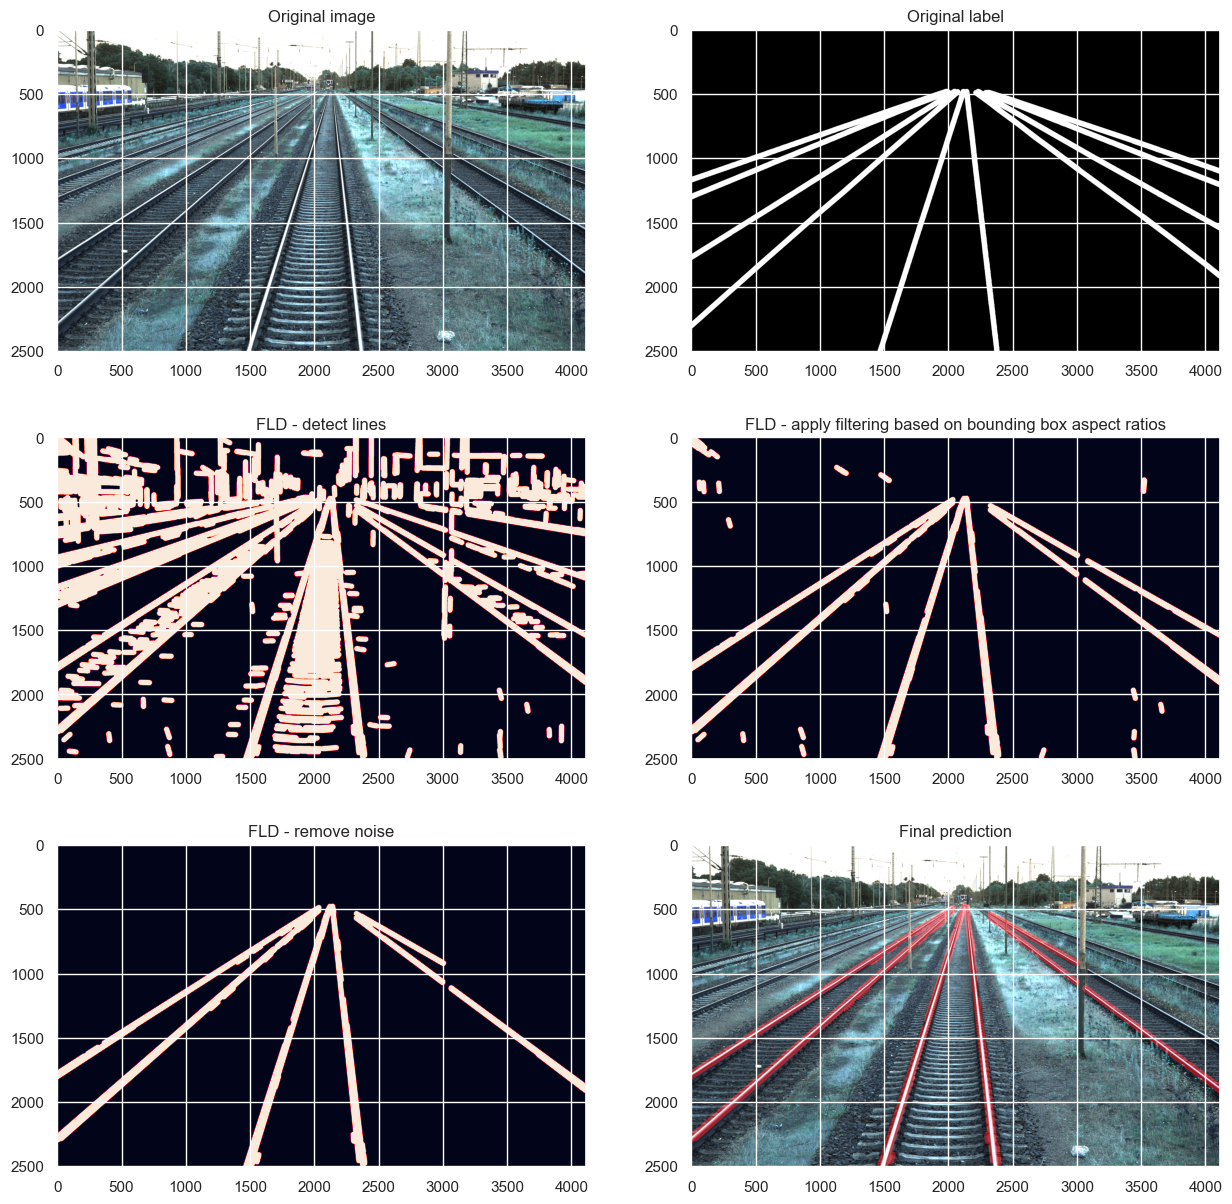
\includegraphics[width=0.9\textwidth]{images/fld/fld_demo}
\caption{Baselining approach based on fast line detection and post-processing. }
\label{fig:fld_demo}
\end{figure}


\subsection{Parameter tuning} \label{sec:fld_parameter}

The performance of our traditional rail detection algorithm depends on a number of parameters. In order to choose the best parameter setting for each combination of sensor and orientation, we tune the parameters according to the grid search technique. Grid search involves specifying a grid of parameter values and exhaustively evaluating the performance of the algorithm for each combination of values. The parameter combination that yields the best performance is selected. Grid search is a simple technique that thoroughly   explores the parameter space but it is also computationally expensive in multi-dimensional spaces.

In total, we test 22.680 parameter settings on 196 images\footnote{The idea is to select one image for each combination of sensor, sensor orientation, and video sequence in the train set (i.e., $3\times3\times33 = 297$). However, there are combinations with no track labels.} from the OSDaR23 dataset. The images are sampled randomly from the train set such that there is one image per sensor per video sequence. 
 
\begin{table}[htbp]
    \centering
    \tiny
    \caption{Sensor Parameters}
    \label{tab:sensor_parameters_fld}
    \begin{tabular}{|l|l|l|}
        \hline
        \textbf{Parameter} & \textbf{Description} & \textbf{Values} \\
        \hline
        Sensors & Combination of sensor and orientation & rgb\_highres\_left, rgb\_highres\_right, rgb\_highres\_center,  \\
                & & rgb\_left, rgb\_right, rgb\_center, ir\_left, ir\_right, ir\_center \\
                 & &  ir\_left, ir\_right, ir\_center \\
        \hline
        Kernel & Kernel for Gaussian blur & 0, 3, 5, 7 \\
        \hline
        Length Threshold & Segment shorter than this will be discarded & 25, 50, 100, 200, 300 \\
        \hline
        Canny Threshold 1 & First threshold for hysteresis procedure in Canny;  & 5, 10, 20, 50, 100, 150 \\
         & second threshold is threshold 1 times 3 &  \\
        \hline
        Aspect Ratio Quantile & Filtering out lines with depending on bounding  & 1, 5, 10 \\
          &  box aspect ratio quantile &  \\
        \hline
        Noise Threshold & Removing small segments that are classified as noise & 0.0, 0.05, 0.1, 0.15, 0.2, 0.25, 0.3 \\
        \hline
    \end{tabular}
\end{table}


Table~\ref{tab:sensor_parameters_fld} presents the best parameter configurations based on the average Dice score. The varying parameter settings across different sensors demonstrate the algorithm's sensitivity to the selected parameters.
The left-oriented camera images seem to benefit from a higher level of blurring with a kernel size of seven. 
The filtering criteria for lines with uncharacteristic bounding box aspect ratios appear to be relatively loose in most cases -- only the most extreme outliers are being removed. Left and right-oriented high-resolution camera images, on the other hand, seem to require a more restrictive filtering. 
The "Avg. Time" column indicates the average inference time in seconds. The inference times seem to be strongly correlated with the entropy metrics discussed in Section~\ref{sec:entropy}; higher entropy values tend to be associated with longer inference times.


\begin{table}[htbp]
\footnotesize
    \centering
    \begin{tabular}{|l|c|c|c|c|c|c|c|}
        \hline
        \textbf{Sensor} & \textbf{Kernel} & \textbf{Length}  & \textbf{Aspect Ratio } & \textbf{Canny } & \textbf{Canny } & \textbf{Noise} & \textbf{Avg. Time } \\
         &  & \textbf{Threshold} & \textbf{Quantile} & \textbf{Th1} & \textbf{Th2} & \textbf{Threshold} & \textbf{(sec)} \\
        \hline
        rgb\_highres\_center & 5 & 50 & 1 & 50 & 150 & 0.25 & 0.052 \\
        rgb\_highres\_right & 0 & 100 & 5 & 10 & 30 & 0.25 & 0.074 \\
        rgb\_center & 3 & 100 & 1 & 10 & 30 & 0.2 & 0.014 \\
        rgb\_highres\_left & 7 & 50 & 5 & 50 & 150 & 0.25 & 0.069 \\
        rgb\_right & 3 & 50 & 1 & 5 & 15 & 0.1 & 0.032 \\
        ir\_left & 7 & 25 & 1 & 5 & 15 & 0.2 & 0.003 \\
        rgb\_left & 7 & 100 & 1 & 20 & 60 & 0.25 & 0.026 \\
        ir\_center & 3 & 25 & 1 & 5 & 15 & 0.2 & 0.003 \\
        ir\_right & 5 & 25 & 1 & 10 & 30 & 0.2 & 0.004 \\
        \hline
    \end{tabular}
      \caption{Best parameter settings and associated performance metrics.}
    \label{tab:sensor_parameters}
\end{table}




\section{Deep-learning based segmentation}

In this section, we will describe the deep-learning based segmentation approach in more detail. The applied model is YOLOv8 which is the latest version of YOLO models by \cite{Jocher_Ultralytics_YOLO_2023}.  YOLOv8 is distributed under the GNU General Public License, which authorizes the users to freely share, modify and distribute the software. The accessibility of the code as well as high performance on many applications led to a large community and much resources for developing and tuning YOLO models. 

YOLOv8 is used to detect objects in images with a single forward pass through the network. The models are pre-trained on large datasets like COCO and ImageNet which enables the prediction of everyday objects \citep{Krishnakumar}. By following the transfer learning technique, the  model can be fine-tuned on new datasets related to the problem at hand (i.e., rail track detection).
The model architecture is presented in Appendix~\ref{app:yolo}.
YOLOv8-Seg model is an extension of the YOLOv8 object detection model that performs semantic segmentation of the input image. The  model has been shown to achieve state-of-the-art results on a variety of object detection and semantic segmentation benchmarks while maintaining high speed and efficiency \citep{Krishnakumar}. 

YOLOv8-seg uses a weighted loss function comprising bounding box loss, objectness loss, and segmentation loss \citep{loss_function}. Bounding box loss calculates the error between the geometry of the predicted and the ground truth box. It is a measure of how well the model predicts the size and location of the bounding boxes. Objectness loss determines how confident the model is about the presence of an object in the bounding box. It compares the probability of an object being present in the prediction with the ground truth value.
Finally, segmentation loss quantifies how close the predicted segmentation map is to the ground truth map. It measures how effectively the model performs the semantic segmentation task.


\subsection{Models}

In order to identify the best model setup for the rail track detection task, we experiment with 18 different models that are validated against different datasets. The models differ in the data the model is trained on, the size of the input image, and the labeling approach. All models are trained for at most 300 epochs. However, the optimization process stops if there has been no improvement in the last 50 epochs. 
Hyper-parameters are either set to default values or automatically chosen in the initialization phase by YOLO.

Table~\ref{tab:training} summarizes the setup of the different models. 
The ``Epochs'' column gives the actual number of performed epochs and ``Duration'' is the wall-clock time for the training process with unified labels and separate labels, respectively. The remaining specifications in the table are the same regardless of the labeling approach. 
The column ``Train Set'' gives the set of images that are used to train the model. ``Image Size'' is either set to 640 or 1280 in order to assess the influence of the image size in the prediction results; the model resizes the input image such that the larger dimension is scaled to the given number of pixels while maintaining the original aspect ratio (e.g., if image size is set to 640 then the RGB low-resolution images are resized from 2464x1600 to 640x416 as the image length and width have to be a multiples of 32).
The batch size is selected automatically by YOLO such that the model can best utilize the available GPU memory without running into ``out of memory'' situations. The ``Optimizer'' column gives the optimization algorithms used for training the neural networks. The optimizer is selected automatically.  SGD (Stochastic Gradient Descent) is a basic optimization algorithm used to minimize the loss function during the training of neural networks. In each iteration, SGD randomly selects a subset of training examples (also referred to as mini-batch) to compute the gradient estimate which supports faster convergence \citep{bottou2010large}. AdamW (Adam with Weight Decay) is a variant of the Adam optimizer that includes an additional term for weight decay regularization. AdamW combines the advantages of both Adam and weight decay regularization which helps prevent overfitting by penalizing large parameter values \citep{kingma2014adam}. 
 

 
\begin{table}[htbp]
    \centering
    \tiny
    \begin{tabular}{|l|c|c|c|c|c|c|c|}
    \hline
    &  &  & & \multicolumn{2}{c|}{\textbf{Unified labels}}   & \multicolumn{2}{c|}{\textbf{Separate labels}}   \\ \cline{5-8}
    \textbf{Train Set} & \textbf{Image Size} & \textbf{Batch Size} & \textbf{Optimizer} & \textbf{Epochs} & \textbf{Duration (HH:MM:SS)} & \textbf{Epoch} & \textbf{Duration (HH:MM:SS)} \\
    \hline
    OSDaR23 RGB & 640 & 23 & AdamW & 121 & 00:37:57 & 93 & 00:35:29 \\
    OSDaR23 infrared & 640 & 23 & AdamW & 196 & 00:51:51 & 223 & 01:01:10 \\
    OSDaR23 RGB & 1280 & 5 & AdamW & 117 & 01:39:58 & 247 & 03:54:41 \\
    OSDaR23 RGB + Railsem19 & 640 & 23 & SGD & 138 & 02:44:37 & 300 & 08:45:13 \\
    OSDaR23 high-res & 1280 & 5 & AdamW & 81 & 04:20:46 & 119 & 17:36:20 \\
    OSDaR23 high-res + Railsem19 & 640 & 23 & SGD & 110 & 13:36:26 & 300 & 60:03:41 \\
    OSDaR23 high-res & 640 & 23 & AdamW & 130 & 13:53:44 & 285 & 43:27:41 \\
    All OSDaR23 & 640 & 23 & SGD & 189 & 23:27:11 & 172 & 36:45:33 \\
    All OSDaR23 + Railsem19 & 640 & 23 & SGD & 224 & 23:42:53 & 300 & 64:51:24 \\
    \hline
    \end{tabular}
    \caption{Training details}
    \label{tab:training}
\end{table}
 
When looking at the table, it becomes apparent that the size of the input images has a large impact on the batch size. With an image size of $640$, 23 images can be processed per iteration. If the image size is set to $1280$ pixels, only 5 images can be processed at once with the given computational resources. The automatic selection of optimizers seems to depend on whether or not the Railsem19 images are added to the train set. With Railsem19 data, YOLO selects the SGD optimizer, without Railsem19 data the AdamW optimizer is used.   
In terms of computational time, it appears that the high-resolution images significantly influence the duration of processing. Among the experiments with an image size of $640$, the presence of high-resolution images in the training set causes at least a five-fold increase in the computation time per epoch. The labeling approach is another factor that has a large effect on the computational time; training the model with all images (OSDaR23 and RailSem19) with separate labels took almost three days whereas the training with unified labels stopped after less than a day.
Also all models with unified labels stopped early as no improvement was observed for 50 epochs. With separate labels  the maximum number of iterations was reached in models that incorporated the RailSem19 dataset. 

Figure~\ref{fig:yolo_models}, presents the results of the experiments with unified labels on the left and with separate labels on the right. On the y-axis, we list the nine models introduced above. The x-axis shows the validation sets on which the models are tested. The models are compared based on the average Dice score.

 The model that performs best on all OSDaR23 images is data\_all\_railsem\_640, on OSDaR23 high-resolution and low-resolution images data\_highres\_railsem\_640 and on OSDaR23 infrared images data\_all\_640 with unified labels and  data\_all\_railsem\_640 with separate labels. This means that all models benefited from adding images from the Railsem19 dataset to the training set, except when applied to the infrared images with unified labels. This result comes at no surprise as the Railsem19 dataset comprises a large variety of different images and deep-learning models are known to perform better with more training data. 
 The lack of generalization of the models trained exclusively on the OSDaR23 data becomes apparent when validated against the Railsem19 dataset: the best dice score is 0.35 with the data\_all\_640 model compared to 0.76 with the data\_highres\_railsem\_640 model when labels are unified; with separate labels the difference is 0.44 versus 0.71.

 It is also interesting to observe the models that are validated against infrared images. While all models with unified labels fail to predict tracks in infrared images except of models that are trained on infrared images, models trained exclusively on infrared images can predict tracks in RGB images with a Dice score of 0.3. This indicates that training on infrared images support the prediction on RGB images but not the other way round. The picture is different when each track is labeled separately. Even if the training set does not contain infrared images, tracks can be predicted in infrared images with a dice score of 0.25.

In general, the results clearly indicate that the performance of the segmentation approach depends on the availability of appropriate training data. The comparison between the different labeling approaches is not straight forward because the dice score is calculated differently. We will perform a comparison based on the same metrics in Section~\ref{sec:results}.


 


\begin{figure}
\centering
\begin{subfigure}[t]{.5\textwidth}
  \centering
  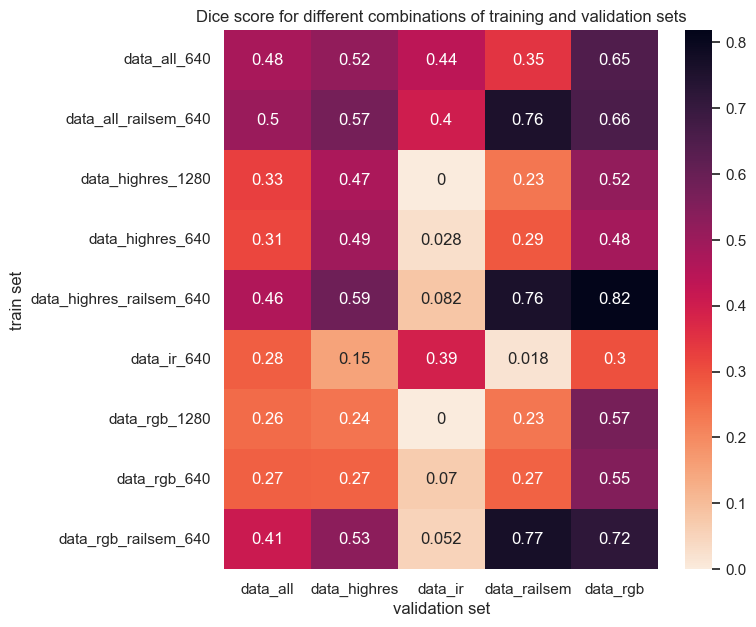
\includegraphics[width=0.9\textwidth]{images/yolo/models}
  \caption{Models with unified labels.}
\end{subfigure}%
\begin{subfigure}[t]{.5\textwidth}
  \centering
  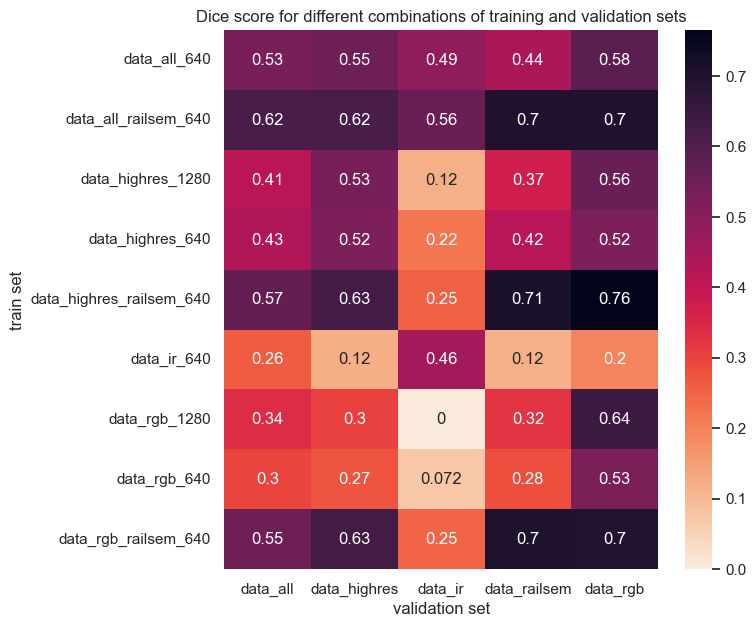
\includegraphics[width=0.9\textwidth]{images/yolo/models_new_label}
  \caption{Models with separate labels. }
\end{subfigure}
\caption{Models with different train and validation set.}
\label{fig:yolo_models}
\end{figure}


The comparison between using 1200 pixel images as input and 600 pixel images reveals that using larger images has no clear advantage on the solution quality. In certain cases (e.g., data\_railsem) the Dice score even decrease when using 1280 pixel images rather than 640 pixel images which might be caused by the smaller batch size that fits into the memory in each training step. What is more, using larger images considerably increases the inference speed which might become a bottle-neck in real-life applications. Table~\ref{tab:inference_speed} show that using large images as input can increase the average inference speed by a factor of around 4. %from under $2 ms$ to around $7 ms$. 

\begin{table}[htbp]
    \centering
    \footnotesize
    \begin{tabular}{|c|cc|cc|}
        \hline
		 & \multicolumn{2}{|c|}{\textbf{Inference speed unified labels [ms]}} & \multicolumn{2}{|c|}{\textbf{Inference speed separate labels [ms]}} \\
        \textbf{Train Set} & \textbf{data\_highres} & \textbf{data\_rgb}  & \textbf{data\_highres} & \textbf{data\_rgb} \\
        \hline
        data\_highres\_1280 & 7.286 & 7.478 & 10.768 & 11.624 \\
        data\_highres\_640 & 1.696 & 1.745 & 4.138 & 3.001 \\
        data\_rgb\_1280 & 5.371 & 6.755 & 8.306 & 8.869 \\
        data\_rgb\_640 & 2.019 & 1.867 & 1.716 & 1.931 \\
        \hline
    \end{tabular}
        \caption{Inference speed in milliseconds}
    \label{tab:inference_speed}
\end{table}

Going forward, we will focus on the models data\_highres\_railsem\_640 and data\_all\_640 with unified labels, and models data\_highres\_railsem\_640 and data\_all\_railsem\_640 with separate labels  for further analysis and refinement as these models provided the best results on the relevant OSDaR23 validation sets. The detailed training results are given in Appending~\ref{app:yolo}.


\subsection{Parameter tuning}

Parameter tuning or hyperparameter tuning refers to the process of selecting the optimal hyperparameters for a neural network model. Hyperparameters cannot be directly learned from the training data but are high-level settings that are provided as an external input to the model. The goal of parameter tuning is to find the combination of hyperparameters that results in the best performance.  Ultralytics YOLO enables hyperparameter tuning by genetic algorithms. 
%Genetic algorithms are inspired by the mechanism of natural selection and genetics based on, e.g., mutation \citep{yolo_parameter}. 

Parameter tuning in YOLO is an iterative process where in each iteration the fitness of the current setting is assessed by training the model for a given number of epochs. We set the number of iterations to 300 and the number of epochs per iteration to 30.  Preliminary experiments revealed that the tuning process is computationally expensive. Therefore, the tuning is performed on 10\% of the training data. 
Table~\ref{tab:model_duration} summarizes the tuning runs with unified labels. %The tuning is very resource intensive 
Despite the reduced training set, the tuning on the high-resolution OSDaR23 images plus Railsem19 images took 146 hours with the SGD optimizer and was aborted after 148 hours with the AdamW optimizer.  

\begin{table}[htbp]
\centering
\footnotesize
\begin{tabular}{|llc|}
\toprule
\textbf{Model} & \textbf{Optimizer} & \textbf{Duration [h]} \\ 
\midrule
\multirow{2}{*}{data\_highres\_railsem\_640} & AdamW & $148^\mathrm{a}$\\
& SGD & $146$ \\
\midrule
\multirow{2}{*}{data\_all\_640} & AdamW & $50$ \\
& SGD & $51$ \\
\bottomrule
\multicolumn{3}{l}{$^{\mathrm{a}}$Tuning run was aborted by the system after 160 iterations.} \\
\end{tabular}
\caption{Parameter tuning with unified labels.}
\label{tab:model_duration}
\end{table}

Table~\ref{tab:tuning_comparison} compares the results with unified labels that are generated by automatically setting the parameters by YOLO, tuning with SGD, and tuning with AdamW. The data\_all\_640 model is used as a basis for the infrared images and data\_highres\_railsem\_640 model is used for the RGB images.
The results indicate that the automatically chosen parameters outperform the tuned parameters on two out of four tests. This is a surprising result but it can probably be explained by the reduced training set that was used during the parameter tuning. For example, if the subset of the training data used for tuning contained less infrared images relative to the entire training set, then the parameters of the data\_all\_640 model would be tuned towards performing better on RGB images. Detailed results of the tuning are given in Appendix~\ref{app:yolo_parameters}.

Given the good overall performance of the automatically tuned parameters and the poor performance of the tuned parameters on the data\_rgb set, we use the models with the automatically chosen parameters for the final analysis.
In the same sense, the parameter tuning was omitted for the models with separate labels. 


\begin{table}[htbp]
\centering
\footnotesize
\begin{tabular}{|l|l|ccc|cc|}
\hline
\textbf{} & \textbf{Validation } & \textbf{  } & \textbf{Dice  } & \textbf{  } & \textbf{SGD vs. } & \textbf{AdamW } \\ 
\textbf{Model} & \textbf{Set} & \textbf{ Auto } & \textbf{Tuned SGD} & \textbf{Tuned AdamW} & \textbf{ Auto [\%]} & \textbf{ Auto [\%]} \\ 
\hline
data\_all\_640 & data\_ir & \textbf{0.440} & 0.425 & 0.375 & -3.324 & -14.704 \\ \hline
\multirow{3}{*}{\shortstack{data\_highres\_\\railsem\_640}} & data\_highres & 0.587 & \textbf{0.596} & 0.558 & 1.480 & -4.913 \\
 & data\_railsem & 0.758 & 0.765 & \textbf{0.766} & 0.879 & 1.057 \\
 & data\_rgb & \textbf{0.818} & 0.774 & 0.752 & -5.440 & -8.140 \\
\hline
\end{tabular}
\caption{Comparison of automatically chosen parameters and tuned parameters based on Dice score with unified labels.}
\label{tab:tuning_comparison}
\end{table}




\chapter{Results} \label{sec:results} % 2000 words

In this section, we analyze the results of the introduced solution approaches and investigate options for post-processing and integration into existing tools for rail-track detection.

\section{Performance analysis}

In this section, we perform a detailed analysis of the proposed solution approaches on the OSDaR23 test set.  The test set is not used during the model development and training process, so the results provide an unbiased performance evaluation on unseen data.
All approaches, FLD, YOLOv8 with unified labels, and YOLOv8 with separate labels are used to predict tracks in the test images. The evaluation is based on the Dice score of the resulting segmentation mask. 

YOLOv8 uses different methods to evaluate the performance during the validation (i.e., on validation set) and prediction (i.e., on test set). The validation method generates detections on padded images, while the predict method does not. This means that the two methods are using slightly different versions of the same image when generating predictions. In order to enable a fair comparison between YOLOv8 and FLD, we evaluate the performance of both approaches by using the same function.

First, we compare the YOLOv8 models with unified labels and with separate labels. Figure~\ref{fig:yolo_vs_yolo} visualizes the distribution of the Dice scores by sensor type and orientation in a violin plot -- a visualization that combines aspects of a box plot and a kernel density plot\footnote{The negative values in the violin plot are caused by the kernel density estimation.} 
Both approaches seem to provide results of similar quality. 
For the left oriented RGB camera and the right oriented high-resolution camera, there is a clear advantage of the separate labeling compared to the unified labeling. For the left oriented infrared camera, the unified labels provide better results.

As both models perform similarly well, we continue the analysis on the model with separate labels as this model provides advantages when applying the results in the real-world. 
Figure~\ref{fig:labeling3} illustrates the result of the two labeling approaches. 
On the top, we give the segmentation result when the labels are unified. In this case, the output is a single bounding box and a single mask marking all pixels that are classified as track. On the other hand, the example on the bottom shows the result when the model is trained with separate labels. In this case, the model provides a separate bounding box and mask for each track in the image which makes it easier in interpret the environment.

 

\begin{figure}[h]
\centering
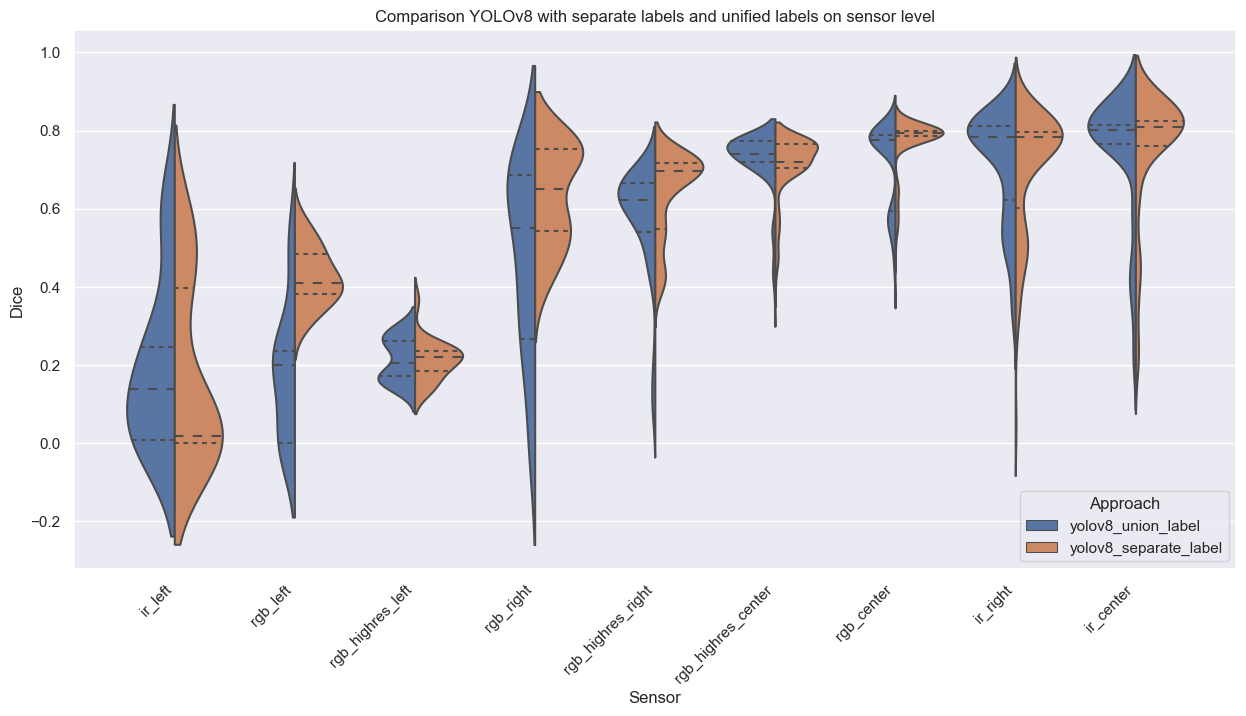
\includegraphics[width=0.9\textwidth]{images/results/violin_plot_yolo}
\caption{Comparison between YOLOv8 models with unified label and separate labels by sensor type. }
\label{fig:yolo_vs_yolo}
\end{figure}


\begin{figure}
\centering
\begin{subfigure}[t]{.5\textwidth}
  \centering
  \includegraphics[width=0.9\textwidth]{images/yolo/example_ul/3_fire_site_3.3_rgb_center_056_1631639533.600000000_segmented}
  \caption{Prediction image with unified labels.}
  \label{fig:labeling_a}
\end{subfigure}%
\begin{subfigure}[t]{.5\textwidth}
  \centering
  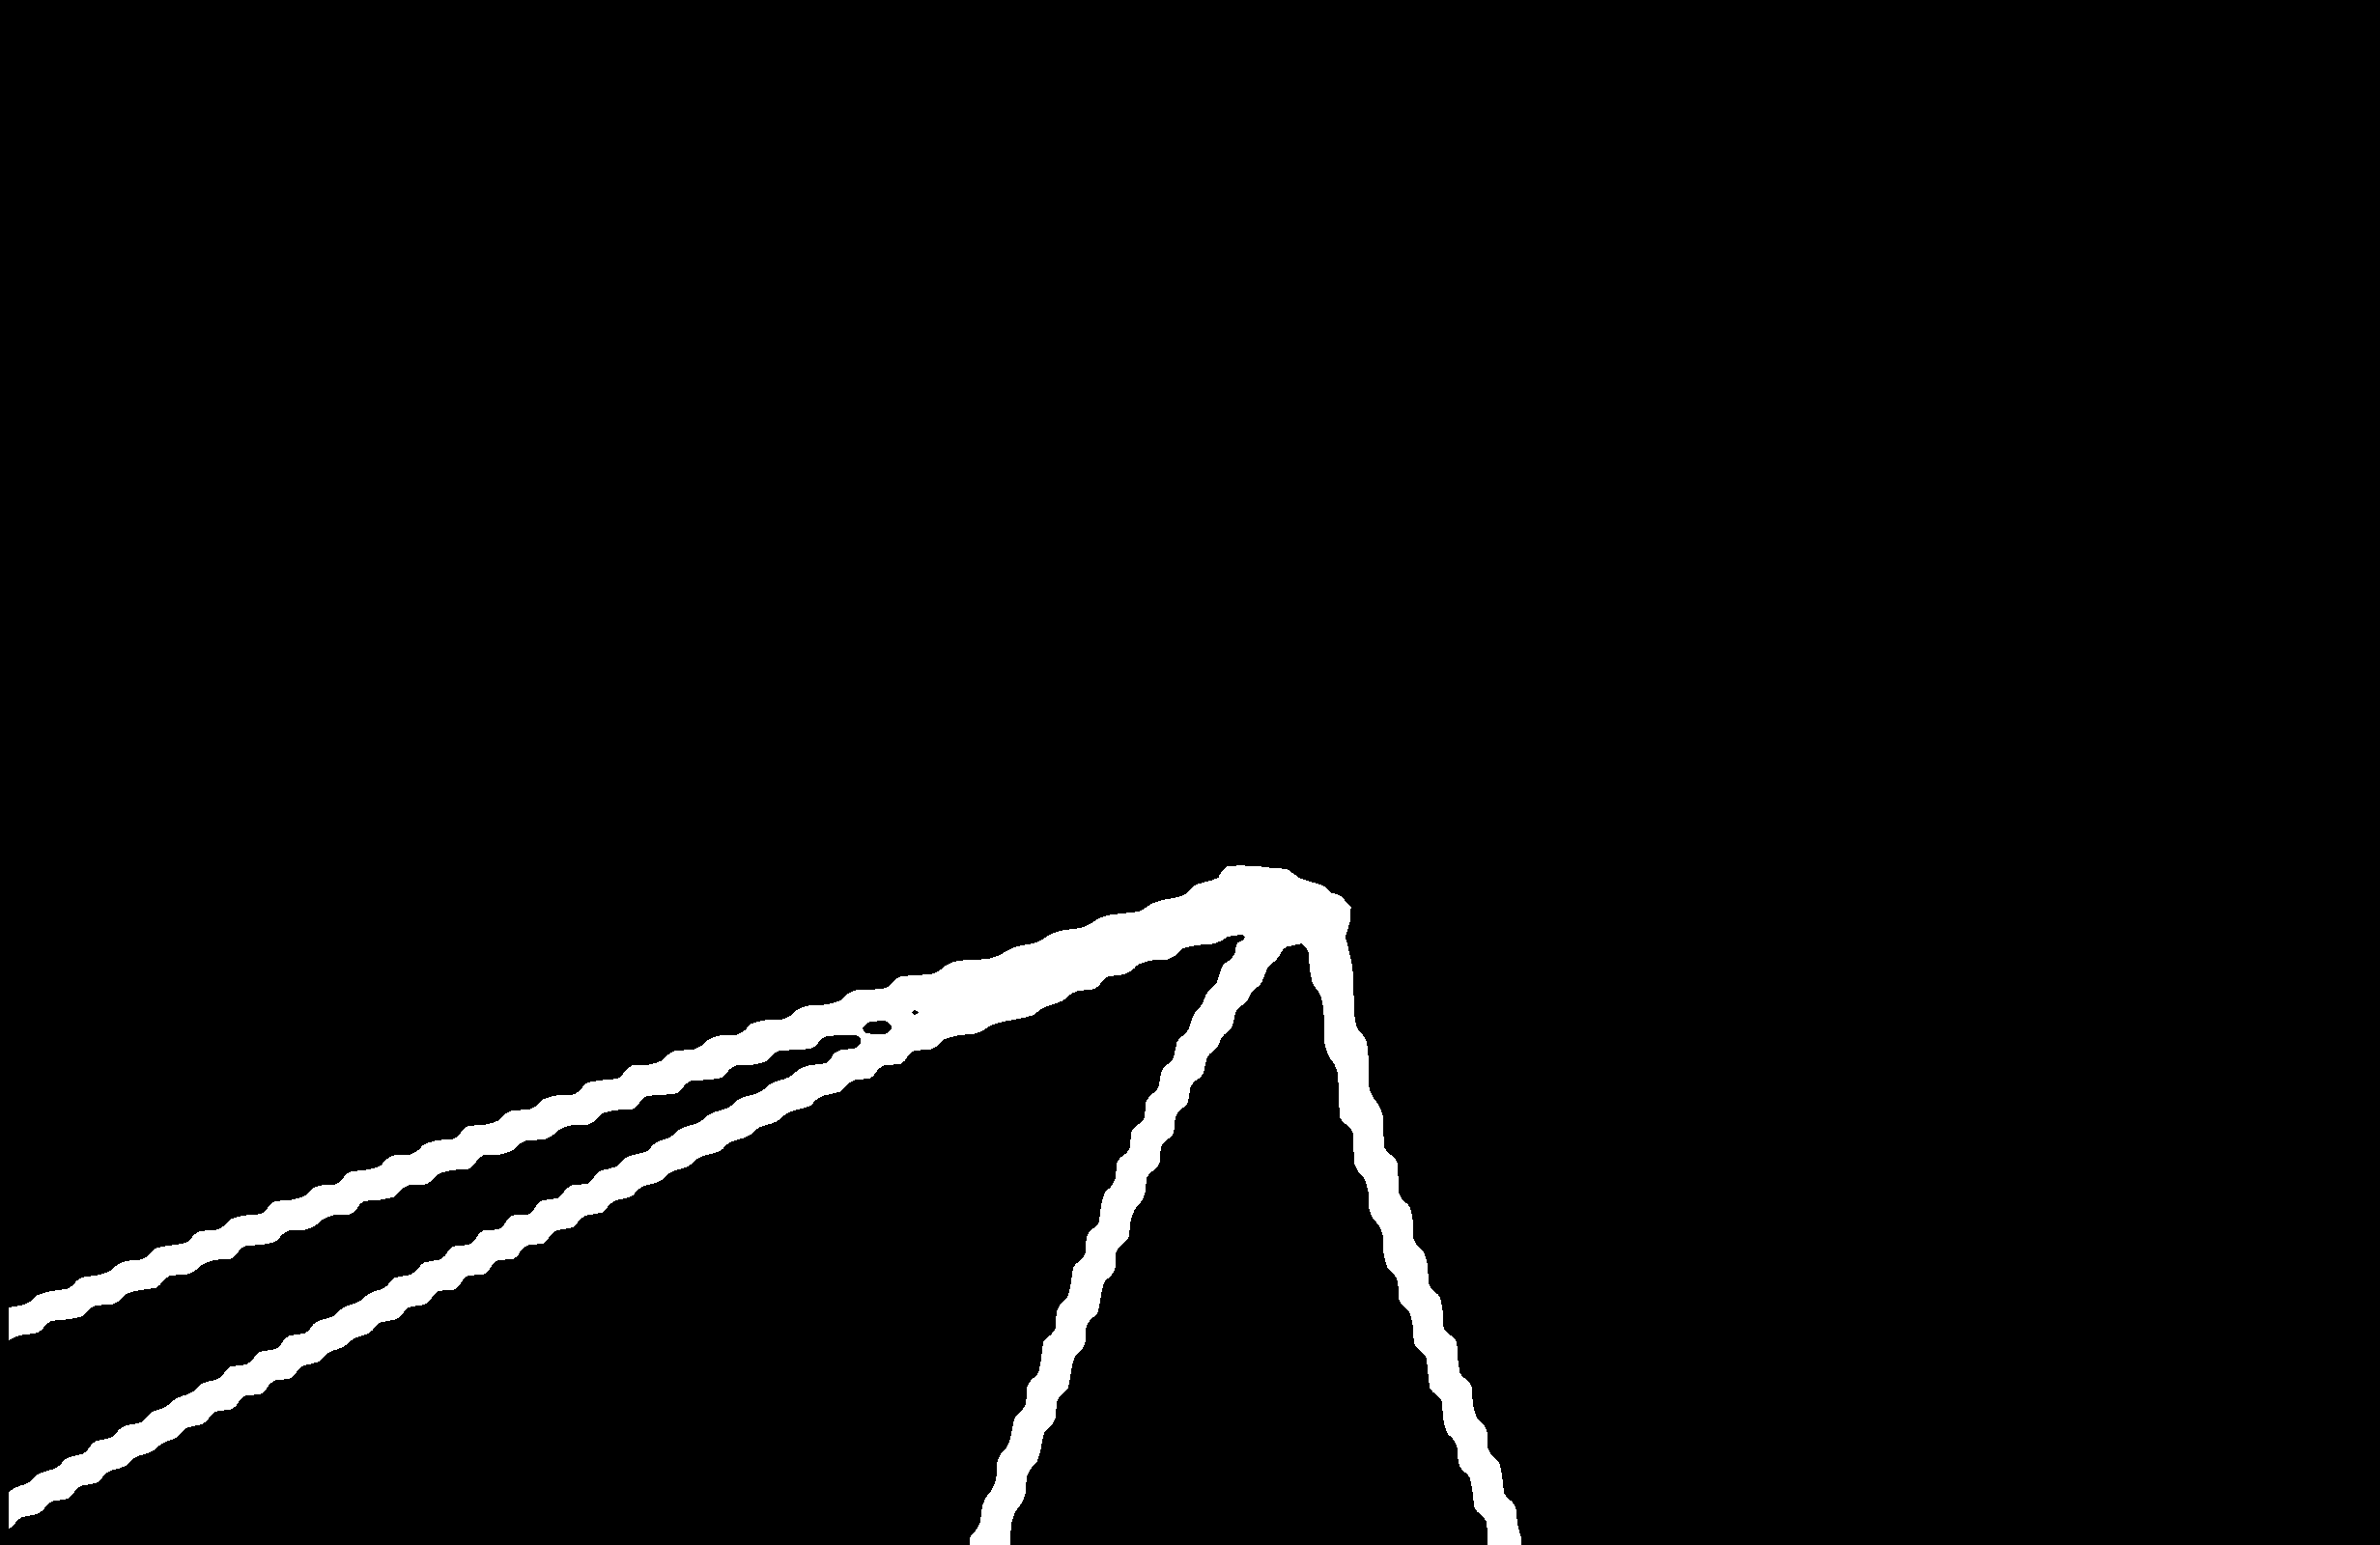
\includegraphics[width=0.9\textwidth]{images/yolo/example_ul/3_fire_site_3.3_rgb_center_056_1631639533.600000000_mask}
  \caption{Prediction mask with unified labels.}
 \label{fig:labeling_b}
\end{subfigure}
\vskip\baselineskip
\begin{subfigure}[t]{.5\textwidth}
  \centering
  \includegraphics[width=0.9\textwidth]{images/yolo/example_sl/3_fire_site_3.3_rgb_center_056_1631639533.600000000_segmented}
  \caption{Prediction image with separate labels.}
 \label{fig:labeling_c}
\end{subfigure}%
\begin{subfigure}[t]{.5\textwidth}
  \centering
  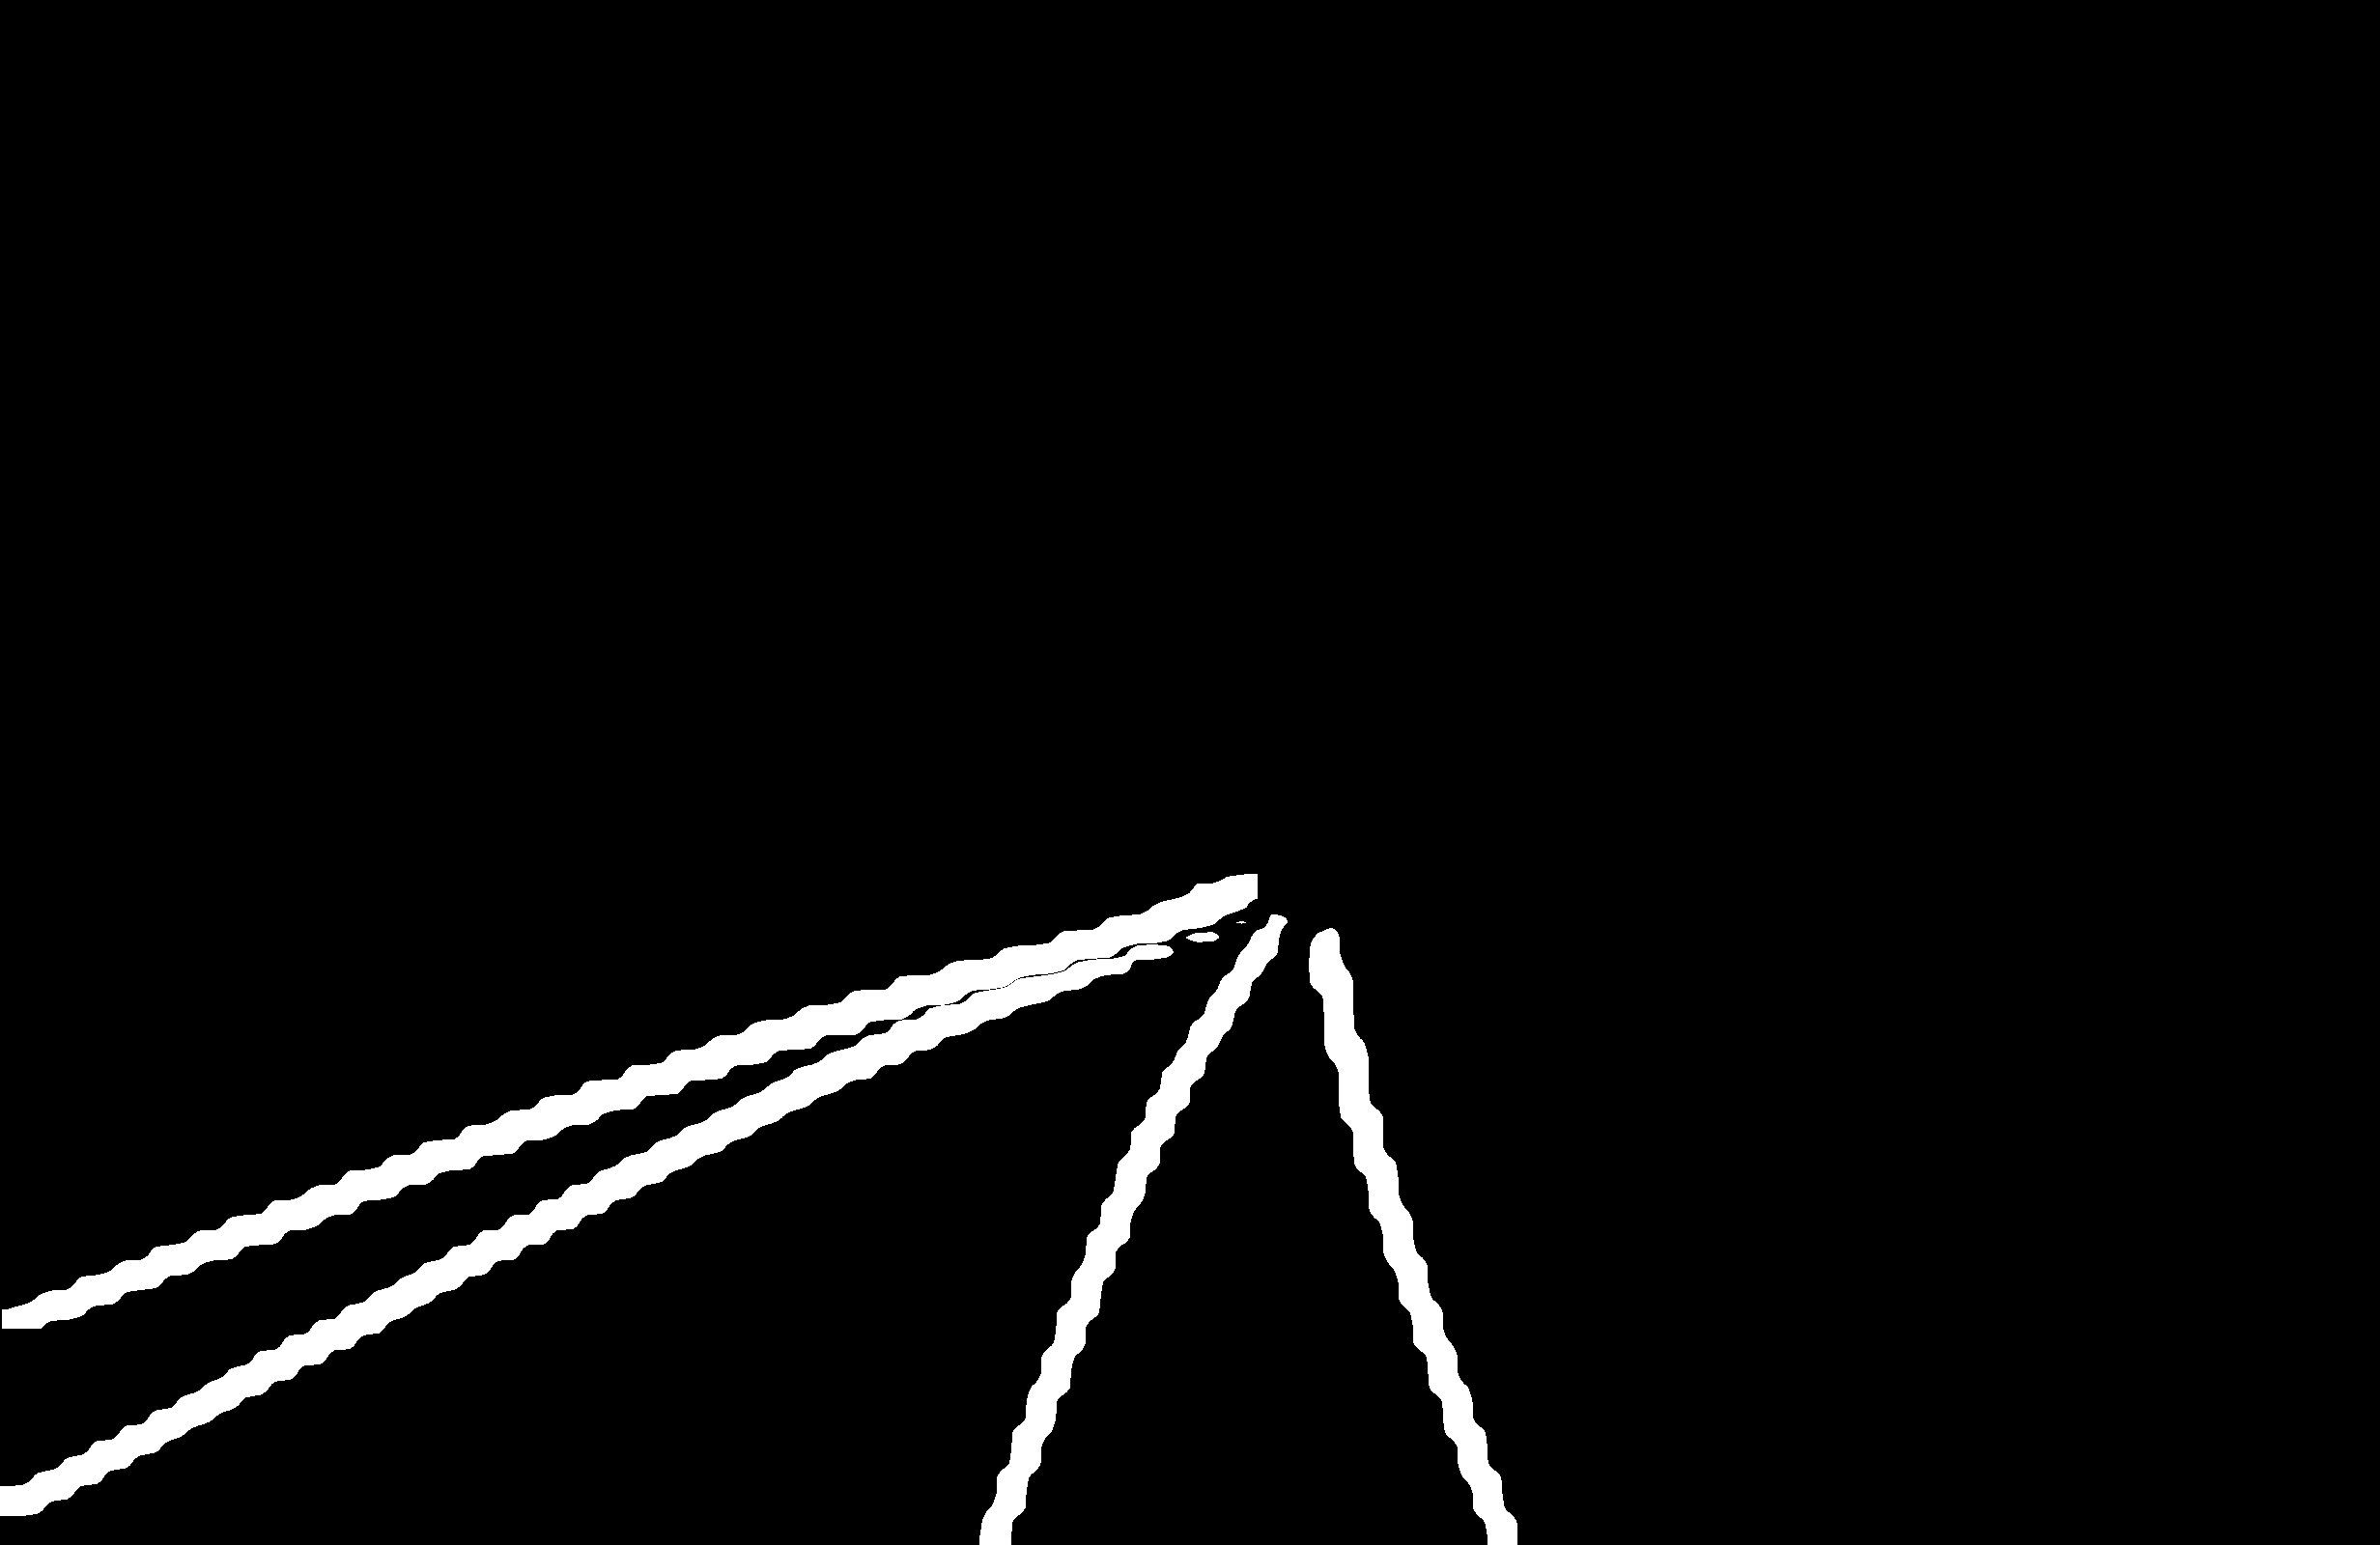
\includegraphics[width=0.9\textwidth]{images/yolo/example_sl/3_fire_site_3.3_rgb_center_056_1631639533.600000000_mask}
  \caption{Prediction mask with separate labels.}
 \label{fig:labeling_d}
\end{subfigure}
\caption{Example results of different labeling approaches.}
\label{fig:labeling3}
\end{figure}




Figure~\ref{fig:yolo_vs_fld} shows the comparison between FLD and YOLOv8 (with separate labels) based on the Dice score where each data point represents one image. The sensor types are distinguished by color. The dashed red line represents the indifference line where scores along this line are the same for YOLOv8 and FLD. If a points is above the line then YOLOv8 performed better on the given image; if a point is below the line, then FLD outperformed YOLOv8. It is easy to see that YOLOv8 performs better than FLD on most images. However, in certain instances FLD achieves better results, e.g., on infrared images. A closer look reveals that most clusters of images where YOLOv8 provides worse predictions than FLD are frames from the same sequence. 
An example is given in Figure~\ref{fig:res_example1}. The ground truth image is given on the left; the labels are colored green\footnote{Note that the labeling is not perfect as certain tracks segments are not marked as tracks}. Predictions by FLD and YOLOv8 are colored red. 
Similarly, the cluster of high-resolution images on which FLD performs better are all frames from the same sequence. The prediction of YOLOv8 and of FLD on one of these frames is given in Figure~\ref{fig:res_example2}
An other interesting observation is that infrared images have the highest Dice scores among all images segmented with YOLOv8. Figure~\ref{fig:res_example4} illustrates the difference between FLD and YOLOv8 on an infrared image.



\begin{figure}[h]
\centering
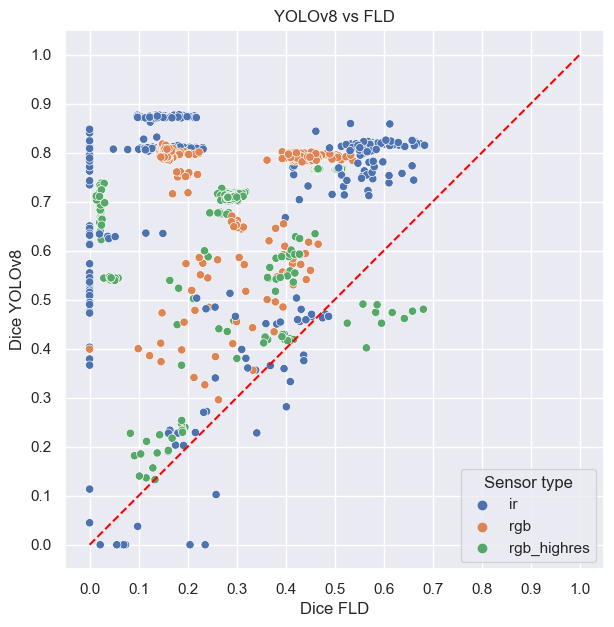
\includegraphics[width=0.8\textwidth]{images/results/dice_fld_vs_yolo_nl}
\caption{Comparison between YOLOv8 (separate labels) and FLD based on Dice score. Sensor types are distinguished by color. }
\label{fig:yolo_vs_fld}
\end{figure}

\begin{figure}
\centering
\begin{subfigure}[t]{.33\textwidth}
  \centering
  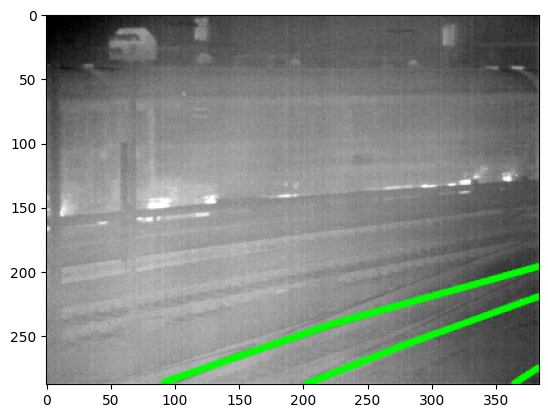
\includegraphics[width=0.9\textwidth]{images/results/example1_gt}
  \caption{Image with ground truth label in green.}
%   \label{fig:bb_long}
\end{subfigure}%
\begin{subfigure}[t]{.33\textwidth}
  \centering
  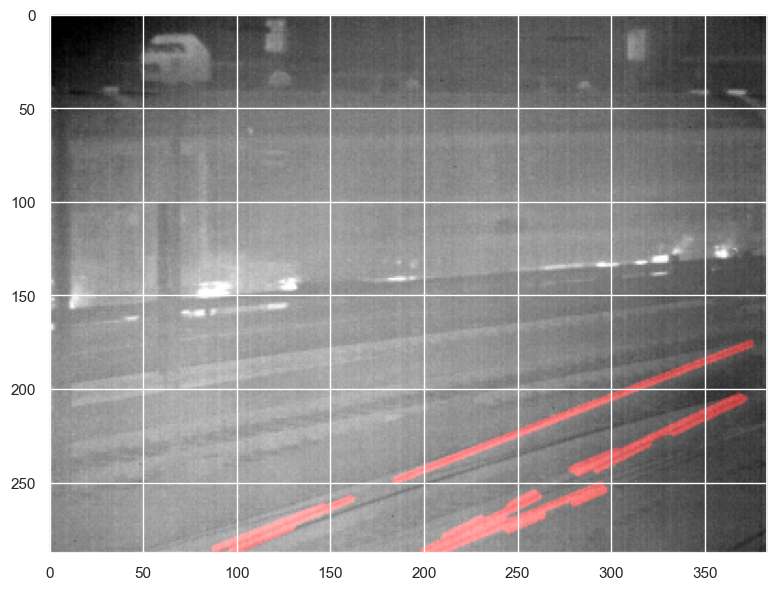
\includegraphics[width=0.9\textwidth]{images/results/example1_fld}
  \caption{FLD provides better prediction for main tracks; the side tracks are only partially segmented.}
%   \label{fig:bb_long}
\end{subfigure}%
\begin{subfigure}[t]{.33\textwidth}
  \centering
  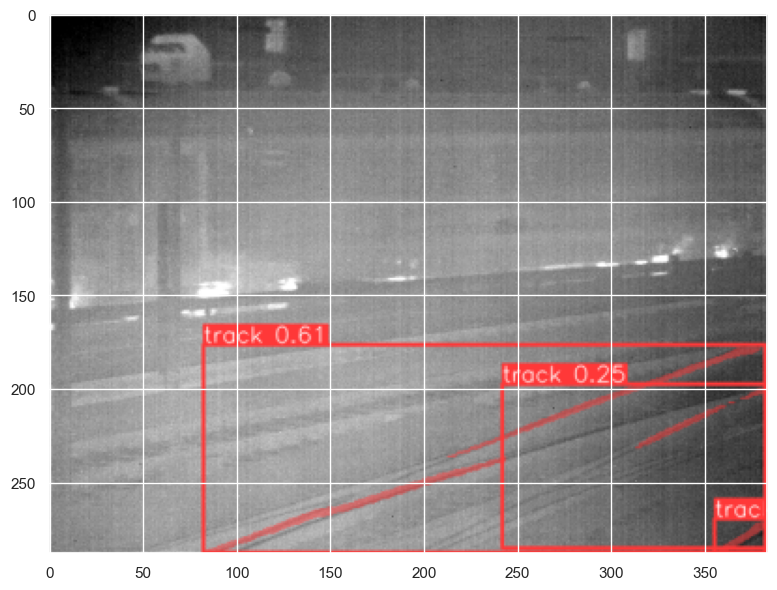
\includegraphics[width=0.9\textwidth]{images/results/example1_yolo}
  \caption{YOLOv8 has many False Negative pixels and low confidence in the result (confidence values are given for each bounding box). }
 % \label{fig:bb_wide}
\end{subfigure}
\caption{Example image where FLD performs better than YOLOv8; predictions are colored red. }
\label{fig:res_example1}
\end{figure}


\begin{figure}
\centering
\begin{subfigure}[t]{.33\textwidth}
  \centering
  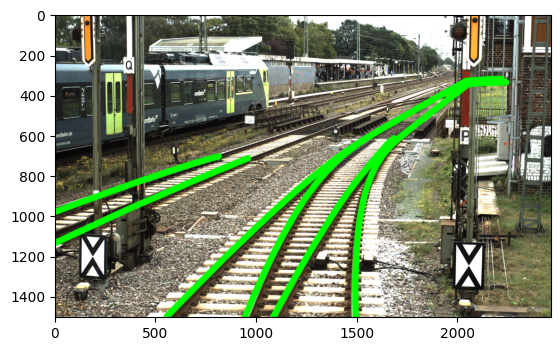
\includegraphics[width=0.9\textwidth]{images/results/example2_gt}
  \caption{Image with ground truth label in green.}
 % \label{fig:bb_wide}
\end{subfigure}
\begin{subfigure}[t]{.33\textwidth}
  \centering
  \includegraphics[width=0.9\textwidth]{images/results/example2}
  \caption{FLD provides good prediction for main tracks; the side tracks are only partially segmented.}
%   \label{fig:bb_long}
\end{subfigure}%
\begin{subfigure}[t]{.33\textwidth}
  \centering
  \includegraphics[width=0.9\textwidth]{images/results/example3}
  \caption{YOLOv8 has many False Negative pixels -- confidence values are given for each bounding box. }
 % \label{fig:bb_wide}
\end{subfigure}
\caption{Example where FLD slightly outperforms YOLOv8.}
\label{fig:res_example2}
\end{figure}




\begin{figure}
\centering
\begin{subfigure}[t]{.33\textwidth}
  \centering
  \includegraphics[width=0.9\textwidth]{images/results/example_4_gt}
  \caption{Image with ground truth label in green.}
%   \label{fig:bb_long}
\end{subfigure}%
\begin{subfigure}[t]{.33\textwidth}
  \centering
  \includegraphics[width=0.9\textwidth]{images/results/example_4_fld}
  \caption{FLD approach cannot detect tracks efficiently in the example image.}
%   \label{fig:bb_long}
\end{subfigure}%
\begin{subfigure}[t]{.33\textwidth}
  \centering
  \includegraphics[width=0.9\textwidth]{images/results/example_4_yolo}
  \caption{YOLOv8 provides precise segmentation with high confidence. }
 % \label{fig:bb_wide}
\end{subfigure}
\caption{Extreme example where YOLOv8 clearly outperforms FLD.}
\label{fig:res_example4}
\end{figure}


In Section~\ref{sec:fld_parameter}, we have seen that the image entropy has an effect on the computation time. In Figure~\ref{fig:dice_vs_entropy}, we examine the relation between Dice and entropy score; the solution approaches are distinguished by color. There is no clear trend in the scatter plot, i.e., there is no linear relationship between Dice score and entropy. However,  both approaches seem to struggle with low entropy images that have uniform intensity  (e.g., which might be the case with infrared images -- see Figure~\ref{fig:entropy_sub1}).
Figure~\ref{fig:dice_vs_brightness} shows the relation between image brightness and the dice score achieved by FLD and YOLOv8, respectively.  Image brightness does not seem to have a significant effect on the result. Even in very dark images YOLOv8 is able to generate predictions with dice scores of around 0.8. 

\begin{figure}[h]
\centering
\includegraphics[width=0.9\textwidth]{images/results/dice_vs_entropy_nl}
\caption{Dice scores vs. entropy scores -- FLD and YOLOv8 are distinguished by color.  }
\label{fig:dice_vs_entropy}
\end{figure}

\begin{figure}[h]
\centering
\includegraphics[width=0.9\textwidth]{images/results/dice_vs_brightness_nl}
\caption{Dice scores vs. brightness scores -- FLD and YOLOv8 are distinguished by color.  }
\label{fig:dice_vs_brightness}
\end{figure}



Figure~\ref{fig:yolo_models}, evaluates and compares FLD and YOLOv8 on a sensor level. 
The Dice scores are visualized in a violin plot.
The Figure supports the conclusion from Figure~\ref{fig:yolo_vs_fld}: YOLOv8 performs better than FLD in most of the cases. YOLOv8 performs particularly well on infrared images. Good results are achieved with forward-facing sensors. In particular, FLD performs best on forward-facing RGB cameras but performs poorly when the cameras are left or right oriented. YOLOv8 is more robust to the sensor type and orientation. Segmenting tracks on images of left oriented cameras seems to be particularly challenging which might be an outcome of the right-hand traffic principle which is mostly followed in Germany.


\begin{figure}[h]
\centering
\includegraphics[width=0.9\textwidth]{images/results/violin_plot_nl}
\caption{Violin plot indicating the difference between YOLOv8 and FLD on sensor level.  }
\label{fig:yolo_models}
\end{figure}



\section{Post-processing}

In the area of rail track detection, representing the result as a polylines rather than segmentation masks can have several practical advantages such as simplified interpretation of the result. The clear representation in form of an array of points offers a concise depiction of detected rail tracks. Additionally, utilizing polylines reduces data volumes compared to segmentation masks which is advantageous if the bandwidth of computational resources is limited. Furthermore, polylines facilitate further processing in subsequent tasks such as detecting obstacles the might block the tracks. 

Training the model with separate labels for each track allows us to identify tracks individually in a post-processing step. Each mask is converted into one polyline by applying a traditional line detector.  
Figure~\ref{fig:postprocessing1} illustrates the idea. The image on the left shows the original input with the overlayed mask given in red. The image in the middle shows the segmentation mask which is generated by combining the four individual masks -- one for each track. The image on the right displays the result where each track is marked by a polyline with a different color.


\begin{figure}
\centering
\begin{subfigure}[t]{.33\textwidth}
  \centering
  \includegraphics[width=0.9\textwidth]{images/postprocessing/9_station_ruebenkamp_9.1_rgb_center_082_1631711160.300000056_segmented}
  \caption{Segmented image.}
%   \label{fig:bb_long}
\end{subfigure}%
\begin{subfigure}[t]{.33\textwidth}
  \centering
  \includegraphics[width=0.9\textwidth]{images/postprocessing/9_station_ruebenkamp_9.1_rgb_center_082_1631711160.300000056_mask}
  \caption{Segmentation mask comprising four tracks.}
%   \label{fig:bb_long}
\end{subfigure}%
\begin{subfigure}[t]{.33\textwidth}
  \centering
  \includegraphics[width=0.9\textwidth]{images/postprocessing/9_station_ruebenkamp_9.1_rgb_center_082_1631711160.300000056_line}
  \caption{Each track can be identified separately. }
 % \label{fig:bb_wide}
\end{subfigure}
\caption{Lines. }
\label{fig:postprocessing1}
\end{figure}




\section{Integration into existing tools}

The ultimate goal of the proposed solution approaches is to integrate the image segmentation model into a live video stream.

Once the image segmentation model has been trained, the camera output is fed into the model. Each frame of the video stream is preprocessed to meet the input requirements of the segmentation model (e.g., the image resized). The frames are then analyzed by the segmentation model to obtain the segmentation masks and labeled regions. 
The segmentation masks can be overlayed onto the original video frames to visualize the segmentation results and the processed frames can be displayed in real-time. Alternatively, the masks can be used as an input into existing rails track detection approaches.

As a proof of concept, we integrate the YOLOv8 model with a rail track analysis algorithm proposed by \cite{danieles_algorithm}. The pseudocode of the algorithm is given in Algorithm~\ref{alg:track_analysis}.

The first step is to capture the frames of the video stream (line 2). Each frame is preprocessed and analyzed by the YOLO model, resulting in a segmentation mask and an image with the segmentation overlay (line 3). The mask and the camera setup are used to generate a bird-eye view of the image by applying the homography technique (line 4). 
Homography is the process of transforming images taken from the camera's perspective to a common coordinate system where the scene is viewed from above (e.g., as if the camera was positioned directly overhead).
In order to generate the bird-eye view, it is essential to calibrate the camera by estimating parameters such as focal length, principal point, and lens distortion coefficients. This information is essential for accurately mapping points between the images and the new coordinate system. Once the camera is calibrated, the homography matrix can be estimated to transform the points between the camera images and the bird-eye view.
The bird-eye view of the mask is then used to extract potential lines that might refer to rail tracks (line 5). There are different approaches to extract lines from the mask. The approach implemented in our experiment is based on finding the contours of the mask, splitting the image into different horizontal segments, calculating the mean point among all points within the contour per segment, and fitting a line through those points. In line 6, we incorporate explicitly available knowledge into the algorithm to analyze the bird-eye-view image and identify the main track and the secondary tracks. For example, the tracks are always parallel from a bird-eye view and the standard gauge (i.e., the distance between the left and the right track) is always $1435mm$. This information is used to exclude false positive segmentation results and pair tracks that belong together.


\begin{algorithm}
\caption{Rail track detection}\label{alg:track_analysis}
\begin{algorithmic}[1]
\Procedure{identify\_tracks}{$video\_stream$, $yolo\_model, camera\_setup$} %\Comment{}
\While{$f \gets \text{capture\_frame}(video\_stream)$}
\State $mask, image\_with\_overlay \gets \text{yolo\_model}(f)$
\State $birdseye\_view \gets \text{apply\_homography}(mask, camera\_setup)$
\State $track\_lines \gets \text{extract\_lines}(birdseye\_view)$
\State $main\_tracks, secondary\_tracks \gets \text{process\_track\_lines}(track\_lines)$
\EndWhile
\State \textbf{return} $main\_tracks, secondary\_tracks$ %\Comment{The gcd is b}
\EndProcedure
\end{algorithmic}
\end{algorithm}


 The process is illustrated in Figure~\ref{fig:postprocessing2}. The image on the left shows the result provided by YOLO. The figure in the middle shows the output of Algorithm~\ref{alg:track_analysis}: based on the segmentation mask, the perspective of the camera is illustrated in magenta; the main tracks are shown in red and the secondary tracks in blue, respectively. The image on the right shows the process of generating the bird-eye view, finding the average contour points (marked by green circles), and fitting potential track lines.



\begin{figure}
\centering
\begin{subfigure}[t]{.395\textwidth}
  \centering
  \includegraphics[width=0.9\textwidth]{images/streaming/img3}
  \caption{Segmented image.}
%   \label{fig:bb_long}
\end{subfigure}%
\begin{subfigure}[t]{.395\textwidth}
  \centering
  \includegraphics[width=0.9\textwidth]{images/streaming/img2}
  \caption{Segmentation mask comprising four tracks.}
%   \label{fig:bb_long}
\end{subfigure}%
\begin{subfigure}[t]{.215\textwidth}
  \centering
  \includegraphics[width=0.9\textwidth]{images/streaming/img1}
  \caption{Each track can be identified separately. }
 % \label{fig:bb_wide}
\end{subfigure}
\caption{Illustration of ``rail track detection'' algorithm. }
\label{fig:postprocessing2}
\end{figure}


Several optimization strategies can be implemented to improve the real-time performance of video processing and enable a seamless segmentation with computationally intensive operations.
For example, parallel processing techniques such as multiprocessing can be utilized to concurrently handle different tasks simultaneously (e.g., segmentation processing, frame capturing, and image preprocessing). 
Hardware acceleration, such as GPU utilization, can significantly speed up inference by leveraging parallel processing capabilities. 
Additionally, selectively skipping frames or processing frames at a lower frequency can reduce the computational load, especially in scenarios with relatively static scenes that often occur on straight tracks. Furthermore, the segmentation model itself can be optimized for faster inference. 






\chapter{Conclusion} % 500 words

This master's thesis addresses a challenge in the area of railway automation. The focus is on multi-sensor rail track detection within the context of Automatic Train Operations (ATO). By leveraging deep learning techniques, particularly semantic segmentation, the study aims to enhance the accuracy and robustness of track detection systems thereby contributing to the efficiency and safety of railway operations.

The research compares deep learning-based segmentation with traditional non-AI-based methods and evaluates the effectiveness of both approaches on different sensor inputs and orientations. By conducting a comprehensive performance evaluation and testing the integrating of the developed model into real-world applications, valuable insights are gained into the feasibility and practical implications of automated track detection systems.

The results demonstrate the advantages of deep learning-based approaches, particularly YOLOv8, over traditional methods in most scenarios. YOLOv8 performs robustly across various sensor types and orientations, with infrared images yielding the highest Dice scores. Furthermore, the results highlight the challenges associated with low entropy images and the impact of sensor orientation on segmentation accuracy. 
Deep-learning approaches have the disadvantage that it is difficult to incorporate expert knowledge. By applying traditional track-detection approaches to post-process the segmentation results, we successfully mitigated false positive classifications and achieved a higher accuracy in identifying tracks.

Overall, this research advances the field of railway automation by providing valuable insights, methodologies, and tools for improving the safety, efficiency, and competitiveness of automatic train operations. The findings provide implications for railway infrastructure management and contribute to the ongoing efforts towards sustainable transportation systems.


Future research could involve applying other deep-learning techniques instead of semantic segmentation. Give the fact that in many cases the desired output are polylines marking tracks, it would be interesting to adjust the YOLinO approach proposed by \cite{meyer2021yolino} for lane detection. %Furthermore, distinguishing the tracks the locomotive occupies currently from the surrounding tracks would support the navigation in the network. 
The approach proposed in this thesis performs well on images from infrared sensors. Therefore, research could focus on more detailed analysis on track detection in adverse weather and low lighting conditions. Another interesting stream of research is the combination of CNNs with recurrent neural network (RNN) architecture designed to model sequential data. Capturing temporal dependencies between video frames  could overcome the limitation of analyzing each frame independently of the sequence in which the frames are generated. Finally, for real-world applications further research could focus on combining traditional segmentation approaches and deep-learning based approaches to increase the overall performance of the system.






%Etwas Text... Hier kommen noch einige Abkürzunge vor zum Beispiel \ac{ABC},\ac{WWW} und \ac{ROFL}.




%%%%%%%%%%%%%%%%%%%%%%%%%%%%%%%%%%%%%%%%%%%%%%%%%%%%%%%%%%%%%%%%%% Hier beginnen die Verzeichnisse.
\clearpage                                                       % Beginne neue Seite

%\printbib                                                        % Literaturverzeichnis LaTeX-Zitier-Standard
%\printbib{Literatur}                                             % Literaturverzeichnis FH-Zitier-Standard
%\printbibliography
\bibliographystyle{plainnat} % We choose the "plain" reference style
\bibliography{Literatur} % Entries are in the refs.bib file

\clearpage

\listoffigures                                                   % Abbildungsverzeichnis
\clearpage

\listoftables                                                    % Tabellenverzeichnis
\clearpage

%\listoflistings                                                  % Quellcodeverzeichnis
%\clearpage
%\phantomsection
%\addcontentsline{toc}{chapter}{\listacroname}
%\chapter*{\listacroname}
%\begin{acronym}[XXXXX]
  %  \acro{ABC}[ABC]{Alphabet}
 %   \acro{WWW}[WWW]{world wide web}
 %   \acro{ROFL}[ROFL]{Rolling on floor laughing}
    
    
    
 %   \acro{ATO}[ATO]{Automatic Train Operations}
 %   \acro{CNN}[CNN]{Convolutional Neural Network}
%\end{acronym}

%%%%%%%%%%%%%%%%%%%%%%%%%%%%%%%%%%%%%%%%%%%%%%%%%%%%%%%%%%%%%%%%%% Hier beginnt der Anhang.
\clearpage


\appendix
\chapter{Appendix}

\section{Sensors used in OSDaR23} \label{app:sensors}

In this thesis, we are focusing on images from the different sensor types. 

\begin{table}[htbp]
  \centering
  \footnotesize
  \begin{tabular}{|l|l|}
    \hline
    \multicolumn{2}{|c|}{\textbf{Three 12MP RGB Cameras}}  \\
    \hline
    Type & Teledyne GenieNano 5GigE C4040  \\
    Sensor data & RGB images (8 Bit, PNG)  \\
    Resolution & 4,112 $\times$ 2,504 px  \\
    Sampling frequency & 10 Hz (synchronized)  \\
    Alignment & trident (in driving direction diagonal left, central and diagonal right)  \\
    \hline
    \multicolumn{2}{|c|}{\textbf{Three 5MP RGB Cameras}}  \\
    \hline
    Type & Teledyne GenieNano C2420  \\
    Sensor data & RGB images (8 Bit, PNG)  \\
    Resolution & 2,464 $\times$ 1,600 px \\
    Sampling frequency & 10 Hz (synchronized)  \\
    Alignment & trident  \\
    \hline
    \multicolumn{2}{|c|}{\textbf{Three IR Cameras}}  \\
    \hline
    Type & Teledyne Calibir DXM640  \\
    Sensor data & Grayscale images (8 Bit, PNG)  \\
    Resolution & 640 $\times$ 480 px  \\
    Sampling frequency & 10 Hz (synchronized)  \\
    Alignment & trident  \\
    \hline
  \end{tabular}
  \caption{OSDaR23 sensor specifications}
  \label{tab:cameras}
\end{table}



\section{Dataset split} \label{app:data_split}

Splitting the OSDaR23 dataset into train, validation, and test subsets is performed based on video sequences. Table~\ref{tab:dataset_split} lists the assignment of sequences to the respective subset. Figure~\ref{fig:data_split} show the split on an image level in total and for each sensor type.

\begin{table}[ht]
\centering
\footnotesize
\begin{tabular}{|l|l|l|}
\hline
\textbf{Train} & \textbf{Validation} & \textbf{Test} \\
\hline
10\_station\_suelldorf\_10.1 & 16\_under\_bridge\_16.1 & 14\_signals\_station\_14.1 \\
11\_main\_station\_11.1 & 18\_vegetation\_switch\_18.1 & 21\_station\_wedel\_21.1 \\
12\_vegetation\_steady\_12.1 & 1\_calibration\_1.2 & 4\_station\_pedestrian\_bridge\_4.2 \\
13\_station\_ohlsdorf\_13.1 & 3\_fire\_site\_3.3 & 4\_station\_pedestrian\_bridge\_4.5 \\
14\_signals\_station\_14.2 & 9\_station\_ruebenkamp\_9.1 & 7\_approach\_underground\_station\_7.2 \\
14\_signals\_station\_14.3 & 9\_station\_ruebenkamp\_9.2 & 8\_station\_altona\_8.3 \\
15\_construction\_vehicle\_15.1 & & \\
17\_signal\_bridge\_17.1 & & \\
19\_vegetation\_curve\_19.1 & & \\
1\_calibration\_1.1 & & \\
20\_vegetation\_squirrel\_20.1 & & \\
21\_station\_wedel\_21.2 & & \\
21\_station\_wedel\_21.3 & & \\
2\_station\_berliner\_tor\_2.1 & & \\
3\_fire\_site\_3.1 & & \\
3\_fire\_site\_3.2 & & \\
3\_fire\_site\_3.4 & & \\
4\_station\_pedestrian\_bridge\_4.1 & & \\
4\_station\_pedestrian\_bridge\_4.3 & & \\
4\_station\_pedestrian\_bridge\_4.4 & & \\
5\_station\_bergedorf\_5.1 & & \\
5\_station\_bergedorf\_5.2 & & \\
6\_station\_klein\_flottbek\_6.1 & & \\
6\_station\_klein\_flottbek\_6.2 & & \\
7\_approach\_underground\_station\_7.1 & & \\
7\_approach\_underground\_station\_7.3 & & \\
8\_station\_altona\_8.1 & & \\
8\_station\_altona\_8.2 & & \\
9\_station\_ruebenkamp\_9.3 & & \\
9\_station\_ruebenkamp\_9.4 & & \\
9\_station\_ruebenkamp\_9.5 & & \\
9\_station\_ruebenkamp\_9.6 & & \\
9\_station\_ruebenkamp\_9.7 & & \\
\hline
\end{tabular}
\caption{Dataset split: OSDaR23 }
\label{tab:dataset_split}
\end{table}



\begin{figure}[h]
\centering
\includegraphics[width=0.9\textwidth]{images/datasets/db/data_split}
\caption{OSDaR23 data split on image level in total and on sensor level. }
\label{fig:data_split}
\end{figure}

\section{Fast line detection}  \label{app:fld}

Table~\ref{tab:sensor_stats} gives the statistics of the aspect ratios of bounding boxes enclosing track labels.


\begin{table}[ht]
\centering
\footnotesize
\begin{tabular}{|c|S[table-format=1.3]|S[table-format=1.3]|S[table-format=1.3]|S[table-format=1.3]|S[table-format=1.3]|S[table-format=1.3]|S[table-format=1.3]|S[table-format=1.3]|}
\hline
\textbf{Sensor} & \textbf{Mean} & \textbf{Median} & \textbf{Q1} & \textbf{Q5} & \textbf{Q95} & \textbf{Q10} & \textbf{Q90} & \textbf{Q99} \\
\hline
ir\_center & 0.714 & 0.379 & 0.104 & 0.113 & 2.210 & 0.126 & 1.857 & 3.917 \\
ir\_left & 1.215 & 1.082 & 0.121 & 0.344 & 2.315 & 0.451 & 2.293 & 2.591 \\
ir\_right & 1.849 & 1.872 & 0.423 & 0.813 & 3.399 & 1.000 & 2.688 & 4.831 \\
rgb\_center & 1.283 & 1.057 & 0.127 & 0.208 & 3.542 & 0.232 & 3.085 & 5.487 \\
rgb\_highres\_center & 0.671 & 0.618 & 0.066 & 0.071 & 1.804 & 0.073 & 1.561 & 2.620 \\
rgb\_highres\_left & 1.320 & 1.120 & 0.138 & 0.654 & 2.192 & 0.738 & 2.181 & 2.578 \\
rgb\_highres\_right & 1.623 & 1.191 & 0.169 & 0.607 & 3.627 & 0.690 & 3.580 & 4.324 \\
rgb\_left & 2.151 & 1.815 & 0.353 & 0.700 & 3.882 & 0.873 & 3.845 & 5.632 \\
rgb\_right & 2.522 & 1.890 & 0.143 & 0.951 & 5.515 & 1.329 & 4.101 & 8.476 \\
\hline
\end{tabular}
\caption{Bounding box aspect ratios for different sensors; Q* denotes quantile.}
\label{tab:sensor_stats}
\end{table}


Figure~\ref{fig:fld_params} shows the effect of different parameters on the performance measured by the Dice score. The results are averaged over 196 images. 

\begin{figure}[h]
\centering
\includegraphics[width=0.9\textwidth]{images/fld/parameter_tuning}
\caption{Heatmap of Dice scores for selected parameter pairs. The Dice scores are average values of 196 images. }
\label{fig:fld_params}
\end{figure}


\section{YOLOv8} \label{app:yolo}

Figure~\ref{fig:yolo_architecture} presents the model architecture of YOLOv8 \citep{RangeKing}.

\begin{figure}[h]
\centering
\includegraphics[width=0.9\textwidth]{images/yolo/architecture}
\caption{Model structure of YOLOv8 detection models. }
\label{fig:yolo_architecture}
\end{figure}

\subsection{Results of data\_highres\_railsem\_640 model with unified labels}

Figure~\ref{fig:training_highres} shows how the performance indicators evolve during the training process, while Figure~\ref{fig:yolo_highres_example} gives and example of a training batch and a validation batch, respectively.
Figure~\ref{fig:mosaic_augmentation_highres} demonstrates the mosaic data augmentation that was introduced in YOLOv8. 
Mosaic data augmentation is a technique where four different images are mixed together and are then provided to the model as input. This technique allows the model to learn the actual objects from different positions and with partial occlusion. 


\begin{figure}[h]
\centering
\includegraphics[width=0.9\textwidth]{images/yolo/highres/results}
\caption{Training results of data\_highres\_railsem\_640 model with unified labels. (B) stands for the results of the bounding box and (M) stands for the result of the segmentation mask.}
\label{fig:training_highres}
\end{figure}

\begin{figure}
\centering
\begin{subfigure}[t]{.5\textwidth}
  \centering
  \includegraphics[width=0.9\textwidth]{images/yolo/highres/train_batch0}
  \caption{Example of training batch.\\ Images are augmented.}
  \label{fig:mosaic_augmentation_highres}
\end{subfigure}%
\begin{subfigure}[t]{.5\textwidth}
  \centering
  \includegraphics[width=0.9\textwidth]{images/yolo/highres/val_batch1_pred}
  \caption{Example of validation batch. }
\end{subfigure}
\caption{Example of training and validation batch during training model data\_highres\_railsem\_640 with unified labels.}
\label{fig:yolo_highres_example}
\end{figure}



\subsection{Results of data\_all\_640 model with unified labels}

Figure~\ref{fig:training_all} shows how the performance indicators evolve during the training process, while Figure~\ref{fig:yolo_all_example} gives and example of a training batch and a validation batch, respectively.
Figure~\ref{fig:validation_batch_1} demonstrates the down-side of having many similar images that are taken from one video sequence -- the validation set is very restricted and therefore not always representative to the wide range of possible scenarios.


\begin{figure}[h]
\centering
\includegraphics[width=0.9\textwidth]{images/yolo/all/results}
\caption{Training results of data\_all\_640 model with unified labels. (B) stands for the results of the bounding box and (M) stands for the result of the segmentation mask.}
\label{fig:training_all}
\end{figure}

\begin{figure}
\centering
\begin{subfigure}[t]{.5\textwidth}
  \centering
  \includegraphics[width=0.9\textwidth]{images/yolo/all/train_batch0}
  \caption{Example of training batch.\\ Images are augmented.}
    \label{fig:mosaic_augmentation_all}
\end{subfigure}%
\begin{subfigure}[t]{.5\textwidth}
  \centering
  \includegraphics[width=0.9\textwidth]{images/yolo/all/val_batch2_pred}
  \caption{Example of validation batch.\\ Images are frames of video sequence.}
  \label{fig:validation_batch_1}
\end{subfigure}
\caption{Example of training and validation batch during training model data\_all\_640 with unified labels.}
\label{fig:yolo_all_example}
\end{figure}

%%%%%%%%%%%%%%%%%

\subsection{Results of data\_highres\_railsem\_640 model with separate labels}

Figure~\ref{fig:training_highres_nl} shows how the performance indicators evolve during the training process, while Figure~\ref{fig:yolo_highres_example_nl} gives and example of a training batch and a validation batch, respectively.
%Figure~\ref{fig:mosaic_augmentation_nl} demonstrates the mosaic data augmentation that was introduced in YOLOv8. 
%Mosaic data augmentation is a technique where four different images are mixed together and provided to the model as input. This technique allows the model to learn the actual objects from different positions and with partial occlusion. 


\begin{figure}[h]
\centering
\includegraphics[width=0.9\textwidth]{images/yolo/highres/results}
\caption{Training results of data\_highres\_railsem\_640 model with separate labels. (B) stands for the results of the bounding box and (M) stands for the result of the segmentation mask.}
\label{fig:training_highres_nl}
\end{figure}

\begin{figure}
\centering
\begin{subfigure}[t]{.5\textwidth}
  \centering
  \includegraphics[width=0.9\textwidth]{images/yolo/highres_nl/train_batch1}
  \caption{Example of training batch.\\ Images are augmented.}
  \label{fig:mosaic_augmentation_highres_nl}
\end{subfigure}%
\begin{subfigure}[t]{.5\textwidth}
  \centering
  \includegraphics[width=0.9\textwidth]{images/yolo/highres_nl/val_batch1_pred}
  \caption{Example of validation batch. }
\end{subfigure}
\caption{Example of training and validation batch during training model data\_highres\_railsem\_640 with separate labels.}
\label{fig:yolo_highres_example_nl}
\end{figure}



\subsection{Results of data\_all\_railsem\_640 model with separate labels}

Figure~\ref{fig:training_all_nl} shows how the performance indicators evolve during the training process, while Figure~\ref{fig:yolo_all_example_nl} gives and example of a training batch and a validation batch, respectively.
Figure~\ref{fig:mosaic_2} demonstrates the down-side of having many similar images that are taken from one video sequence -- the validation set is very restricted and therefore not always representative to the wide range of possible scenarios.


\begin{figure}[h]
\centering
\includegraphics[width=0.9\textwidth]{images/yolo/all_nl/results}
\caption{Training results of data\_al\_railsem\_640 model with separate labels. (B) stands for the results of the bounding box and (M) stands for the result of the segmentation mask.}
\label{fig:training_all_nl}
\end{figure}

\begin{figure}
\centering
\begin{subfigure}[t]{.5\textwidth}
  \centering
  \includegraphics[width=0.9\textwidth]{images/yolo/all_nl/train_batch2}
  \caption{Example of training batch.\\ Images are augmented.}
    \label{fig:mosaic_augmentation_highres_all}
\end{subfigure}%
\begin{subfigure}[t]{.5\textwidth}
  \centering
  \includegraphics[width=0.9\textwidth]{images/yolo/all_nl/val_batch2_pred}
  \caption{Example of validation batch.\\ Images are frames of video sequence.}
  \label{fig:mosaic_2}
\end{subfigure}
\caption{Example of training and validation batch during training model data\_all\_railsem\_640 with separate labels.}
\label{fig:yolo_all_example_nl}
\end{figure}


%%%%%%%%%%%%%%%%%%%%

\subsection{Parameter tuning with unified labels} \label{app:yolo_parameters}

Figure~\ref{fig:yolo_tune_highres_adam} and Figure~\ref{fig:yolo_tune_highres_sgd} visualize the tuning process on the data\_highres\_railsem\_640 model  with AdamW and SGD optimizer, respectively.
The parameters are described in Table~\ref{tab:yolo_parameters}. Certain parameters, such as degrees, translate, etc. are fixed at zero throughout the tuning process as it is unlikely that the resulting images appear in the real-world.


\begin{table}[h]
\footnotesize
\centering
\begin{tabular}{|l|l|}
\hline
\textbf{Parameter} & \textbf{Description} \\ \hline
lr0 & initial learning rate \\ 
lrf & final learning rate \\ 
momentum & SGD momentum/Adam beta1 \\ 
weight\_decay & optimizer weight decay \\ 
warmup\_momentum & warmup initial momentum \\ 
box & box loss gain \\ 
cls & classification loss gain \\ 
dfl & dual focal loss gain \\ 
hsv\_s & image Hue Saturation Value augmentation (fraction) \\ 
hsv\_v & image Hue Saturation Value augmentation (fraction) \\ 
degrees & image rotation (+/- deg) \\ 
translate & image translation (+/- fraction) \\ 
shear & image shear (+/- deg) \\ 
perspective & image perspective (+/- fraction),\\ 
flipud & image flip up-down (probability) \\ 
fliplr & image flip left-right (probability) \\ 
mixup & image mixup (probability) \\ 
copy\_paste & segment copy-paste (probability) \\ \hline
\end{tabular}
\caption{Description of YOLO parameters}
\label{tab:yolo_parameters}
\end{table}

\begin{figure}
\centering
\begin{subfigure}[t]{.5\textwidth}
  \centering
  \includegraphics[width=0.9\textwidth]{images/yolo/highres/adam/tune_scatter_plots}
  \caption{Search space for different parameters. Density is distinguished by color: yellow shades indicate higher density}
\end{subfigure}%
\begin{subfigure}[t]{.5\textwidth}
  \centering
  \includegraphics[width=0.9\textwidth]{images/yolo/highres/adam/tune_fitness}
  \caption{Evolution of fitness value over 160 iterations. Model fitness is a weighted combination of different metrics (e.g., precision, recall, mAP@0.5).}
  \label{fig:images_from_videos}
\end{subfigure}
\caption{Parameter tuning of model data\_highres\_railsem\_640 with AdamW optimizer.}
\label{fig:yolo_tune_highres_adam}
\end{figure}

\begin{figure}
\centering
\begin{subfigure}[t]{.5\textwidth}
  \centering
  \includegraphics[width=0.9\textwidth]{images/yolo/highres/sgd/tune_scatter_plots}
  \caption{Search space for different parameters. Density is distinguished by color: yellow shades indicate higher density}
\end{subfigure}%
\begin{subfigure}[t]{.5\textwidth}
  \centering
  \includegraphics[width=0.9\textwidth]{images/yolo/highres/sgd/tune_fitness}
  \caption{Evolution of fitness value over 300 iterations. Model fitness is a weighted combination of different metrics (e.g., precision, recall, mAP@0.5).}
  \label{fig:images_from_videos}
\end{subfigure}
\caption{Parameter tuning of model data\_highres\_railsem\_640 with SGD optimizer. \\ }
\label{fig:yolo_tune_highres_sgd}
\end{figure}


Figure~\ref{fig:yolo_tune_all_adam} and Figure~\ref{fig:yolo_tune_all_sgd} visualize the tuning process on the data\_all\_640 model  with AdamW and SGD optimizer, respectively.

\begin{figure}
\centering
\begin{subfigure}[t]{.5\textwidth}
  \centering
  \includegraphics[width=0.9\textwidth]{images/yolo/all/adam/tune_scatter_plots}
  \caption{Search space for different parameters. Density is distinguished by color: yellow shades indicate higher density}
\end{subfigure}%
\begin{subfigure}[t]{.5\textwidth}
  \centering
  \includegraphics[width=0.9\textwidth]{images/yolo/all/adam/tune_fitness}
  \caption{Evolution of fitness value over 300 iterations. Model fitness is a weighted combination of different metrics (e.g., precision, recall, mAP@0.5).}
  \label{fig:images_from_videos}
\end{subfigure}
\caption{Parameter tuning of model data\_all\_640 with AdamW optimizer.}
\label{fig:yolo_tune_all_adam}
\end{figure}

\begin{figure}
\centering
\begin{subfigure}[t]{.5\textwidth}
  \centering
  \includegraphics[width=0.9\textwidth]{images/yolo/all/sgd/tune_scatter_plots}
  \caption{Search space for different parameters. Density is distinguished by color: yellow shades indicate higher density}
\end{subfigure}%
\begin{subfigure}[t]{.5\textwidth}
  \centering
  \includegraphics[width=0.9\textwidth]{images/yolo/all/sgd/tune_fitness}
  \caption{Evolution of fitness value over 300 iterations. Model fitness is a weighted combination of different metrics (e.g., precision, recall, mAP@0.5).}
  \label{fig:images_from_videos}
\end{subfigure}
\caption{Parameter tuning of model data\_all\_640 with SGD optimizer. \\ }
\label{fig:yolo_tune_all_sgd}
\end{figure}

%\clearpage
%\chapter{Appendix}
\end{document}
%%%%%%%%%%%%%%%%%%%%%%%%%%%%%%%%%%%%%%%%%%%%%%%%%%%%%%%%%%%%%%%%%% Ende des Inhalts